\documentclass[11pt]{article}
\usepackage[T1]{fontenc}
\usepackage[utf8]{inputenc}
\usepackage{amsmath,amssymb,amsthm,booktabs,longtable,array}
\usepackage[margin=1in]{geometry}
\usepackage{hyperref,xurl}
\usepackage{tikz}
\usetikzlibrary{positioning,arrows.meta}
\newtheorem{theorem}{Theorem}[section]
\newtheorem{proposition}[theorem]{Proposition}
\newtheorem{lemma}[theorem]{Lemma}
\newtheorem{corollary}[theorem]{Corollary}
\theoremstyle{remark}
\newtheorem{remark}[theorem]{Remark}
\newcommand{\HH}{\mathbb H}
\newcommand{\RR}{\mathbb R}
\newcommand{\rk}{\operatorname{rk}}
\newcommand{\En}{\mathcal E}
\newcommand{\CompactBound}{23}
\newcommand{\src}[1]{\path{results/#1}}
\newcommand{\ph}{\varphi}
\title{Farthest vertices and dimension bounds\\
for compact hyperbolic Coxeter polytopes}
\author{Coxeter Polytopes Frontier Project}
\date{20 October 2026}
\begin{document}
\maketitle

\begin{abstract}
We obtain a dimension bound of \CompactBound\ for compact hyperbolic
Coxeter polytopes from estimates at a vertex farthest from an interior
point. One common spatial vector has squared norm less than one, and
its orthogonal projections onto the finite vertex components have
additive costs. Actual opposite walls, positive acute projections,
and feasible timelike combinations give stronger constraints than
edge lengths alone. Every $A_r$, $r\ge7$, costs more than $1/2$,
and every $A_r$, $r\ge17$, costs more than $5/7$.
A localized prefix estimate supplies the complementary cost for
large $B$ and $D$ components. A stronger $A_{20}$ estimate and a
coupled $D_{23}$--$A_1$ argument close the last two patterns.
The component estimates allow arbitrary other finite components at
the chosen vertex, so their costs can be combined in one budget.
Arithmeticity is not required. The argument uses actual walls and
feasible points of the original polytope throughout.
\end{abstract}

\section{Statement and proof strategy}\label{sec:scope}

A compact hyperbolic Coxeter polytope has finitely many facets and
dihedral angles $\pi/m$, $m\ge2$. Its outward unit facet normals lie
in Lorentz space of signature $(n,1)$, and the polytope is given by
$(q,n_i)\le0$ on the future unit hyperboloid.

\begin{theorem}\label{thm:main}
Every compact hyperbolic Coxeter polytope has dimension at most
\CompactBound.
\end{theorem}

The published starting bound is $n\le29$ \cite{Vin84}. We exclude
dimensions $24$ through $29$ by examining one actual finite vertex. The
external geometric and diagram inputs are compact acute simplicity,
the nonpositive products of distinct outward wall normals, finite
spherical Coxeter classification, and the fact that a Lann\'er diagram
has at most five vertices; see \cite{Vin85}. All component estimates
and component exclusions used below are internal arguments.

Sections~\ref{sec:geometry}--\ref{sec:global} give the common geometry,
ordinary costs and debits, complete finite continuation lists, actual
component pressures, prefix argument, and global deduction.
The component propositions are proved here rather than attributed to
the published classification. Appendix~\ref{app:map} gives a guide to
the supporting derivations and the scope of the accompanying
verification material.

The method does not require an arbitrary facet to be a Coxeter
polytope. It also does not replace actual walls by a convenient
abstract Gram completion. Every auxiliary point below satisfies the
inequalities of the entire original polytope.

\subsection{The common argument and its case splits}

The proof starts with one geometric observation, rather than a list
of diagrams. At a farthest vertex, every finite component constrains
the orthogonal projection of the same vector $x$. These squared
projection norms add, and their sum is less than one. The task is
therefore to prove component costs that no sufficiently large
finite forest can afford.

The argument first separates at the component type. Small and
exceptional types admit the ordinary costs of
Proposition~\ref{prop:ordinary}. Large $A$ components require a
coupled analysis of the two ends of a chain, carried out in
Section~\ref{sec:largeA}. Large $B$ and $D$ components instead
admit the coordinate-prefix estimates of Section~\ref{sec:prefix}.
These estimates allow arbitrary other components at the chosen
vertex; a bound for a whole irreducible vertex would not suffice.

The branches reunite in Section~\ref{sec:global}. Its rank and
energy accounting excludes dimensions $25$ through $29$ and leaves
only two patterns in dimension $24$. Those two patterns explain the
last case-specific arguments: the stronger $A_{20}$ cost in
Section~\ref{sec:A20}, and the coupling between $D_{23}$ and its
short isolated spectator in Section~\ref{sec:D23}. They are parts
of this proof, rather than separate dimension-bound papers.

The finite continuation lists used here are mathematical case
analyses. Each needs a proof that its allowed contacts are exhaustive
and that its rejected branches cannot occur. A source hash checks
neither assertion. The proof uses no numerical search or combinatorial
enumeration script: the finite lists are justified by the retained finite diagrams and
explicit affine witnesses before their energy inequalities are used.

\section{One actual vector at a farthest vertex}\label{sec:geometry}

Fix a strict interior future unit point $z$ of a compact polytope
$P$. The function $q\mapsto-(z,q)=\cosh d(z,q)$ is strictly convex
on every geodesic, so a maximum over $P$ occurs at a vertex $p$.
Write
\[
 z=E(p-x),\qquad E=-(z,p)>0,\qquad x\perp p.
\]
Then
\begin{equation}\label{eq:energy}
 \|x\|^2=1-E^{-2}<1.
\end{equation}
The incident normals have a positive definite Gram matrix $B$.
Let $C=B^{-1}$, let $\omega_i=\sum_j C_{ij}n_j$ be the spatial
duals, and put
\[
 d_i=C_{ii},\qquad u_i=\omega_i/\sqrt{d_i}.
\]
The finite diagram is an orthogonal union of irreducible components.
Thus $x=\sum_Tx_T$ and $\|x\|^2=\sum_T\|x_T\|^2$.

The inward direction of edge $i$ is $-u_i$. If its length is $L_i$,
its other endpoint is $p_i=\cosh L_i\,p-\sinh L_i\,u_i$. Farthest
comparison gives
\begin{equation}\label{eq:half}
 x\cdot u_i\ge\tau_i:=\tanh(L_i/2)>0.
\end{equation}
Strict interiority also gives $x\cdot n_i>0$. For an actual outside
unit wall write
\[
 c=A p-v,\qquad A=-(p,c)>0,\qquad \beta_i=-(c,n_i)\ge0.
\]
Its spatial vector is $v=\sum_i\beta_i\omega_i$, with
$A^2=\beta^TC\beta-1$, and
\begin{equation}\label{eq:interior}
 x\cdot v<A.
\end{equation}

\subsection{Positive projections and reciprocal shadows}

A positive definite matrix with nonpositive off-diagonal entries has
entrywise nonnegative inverse. If $J$ is a positive principal set of
actual normals, projecting a strict interior timelike vector onto
$J^\perp$ adds a nonnegative combination of those normals. The
result remains timelike and strictly satisfies every other wall
inequality. Hence a positive principal set defines an actual face.
In particular, a positive full replacement containing an already
actual wall gives an actual finite endpoint.

An affine principal set is impossible in a compact chamber. Its
positive kernel gives a nonzero future null combination with
nonpositive products against every wall. Nonzeroness follows by
pairing with a strict interior point. This would be a feasible ideal
point. These arguments use the all-wall sign in
\cite[p.~42, \S2.1]{Vin85}.

\begin{lemma}[Actual reciprocal shadow]\label{lem:shadow}
For an actual outside wall $c$, put
$v_i=(C\beta)_i/\sqrt{d_i}$ and $T_i=v_i/A$.
If $T_i>1$, the wall $c$ is the actual opposite of edge $i$ and
$\tanh L_i=1/T_i$. If it is not that opposite, then
$\tanh L_i\ge T_i$. The value $T_i=1$ is impossible in the compact
case. Distinct actual opposites satisfy
\begin{equation}\label{eq:pair}
 \tanh L_i\,\tanh L_j\ge
 K_{ij}:=\frac{C_{ij}}{\sqrt{d_id_j}}.
\end{equation}
\end{lemma}
\begin{proof}
The Schur identity says that
$C-C_{\cdot i}C_{i\cdot}/d_i$ is zero on row and column $i$ and
equals the inverse of the retained old Gram elsewhere. It is
entrywise nonnegative. If a different actual opposite has height
$D$ and contacts $\gamma$, acuteness therefore gives
\[
 AD\ge\beta^TC\gamma
 \ge\frac{(C\beta)_i(C\gamma)_i}{d_i}.
\]
Its endpoint equation is
$\tanh L_i=D\sqrt{d_i}/(C\gamma)_i$, proving the alternative.
For $T_i>1$ that alternative is impossible, while the positive
replacement criterion gives the stated actual closure. Equality
gives an ideal rather than finite endpoint. Applying the same
Schur inequality to the actual opposite of $i$ gives
$T_j\ge K_{ij}/\tanh L_i$, and proves \eqref{eq:pair}.
\end{proof}

It is essential that \eqref{eq:pair} uses full tangents.
Write $F(t)=2t/(1+t^2)$. If a component has energy at most $e<1$,
then for a pair of correlation $k$,
\begin{equation}\label{eq:pairupper}
 F(\tau_i)F(\tau_j)
 \le\frac{4s}{(1+s)^2},
 \qquad s=\frac{e(1+k)}2.
\end{equation}
Indeed $\tau_i+\tau_j\le\sqrt{2e(1+k)}$, and $\log F$ is concave
on $(0,1)$. A strict reverse comparison with $k$ forces the same
actual opposite.

\begin{lemma}[Opposites respect whole components]\label{lem:orthogonal}
Two orthogonal outgoing directions cannot share an actual opposite
at a farthest vertex.
\end{lemma}
\begin{proof}
Suppose $i,j$ share $c$ and $u_i\cdot u_j=0$. Clear the other old
normals positively, obtaining $c_F$ in the span of $p,u_i,u_j$.
Strict interiority gives $(z,c_F)<0$. Since both endpoints lie on $c$,
with $r_i=\tanh L_i$ and $r_j=\tanh L_j$,
\[
 c_F=A p-\frac A{r_i}u_i-\frac A{r_j}u_j,
 \qquad \frac{x\cdot u_i}{r_i}+\frac{x\cdot u_j}{r_j}<1.
\]
But \eqref{eq:half} makes the left side at least
$1+(\tau_i^2+\tau_j^2)/2>1$, a contradiction.
\end{proof}

In each retained foreign component an actual opposite has at most
one contact: two would give a cycle in a finite diagram. Its cost
is $q=\beta_j^2C_{jj}\ge1/4$. In a nontrivial component,
$C_{jj}\ge4/3$, so there is no cost in $(1/4,1/3)$.
Moreover
\begin{equation}\label{eq:foreign}
 q<A^2.
\end{equation}
Otherwise Lemma~\ref{lem:shadow} closes the contacted foreign
direction too, contrary to Lemma~\ref{lem:orthogonal}, or gives a
null endpoint in the equality case.

\subsection{Actual finite and timelike core points}

For an old set $J$ let $w=\sum_{j\in J}(B_J^{-1}\beta_J)_j n_j$
and $\delta=1-\beta_J^TB_J^{-1}\beta_J$. Then $w$ has nonnegative
coefficients and $\eta=c+w$ has square $\delta$, products zero on
$J$, and product $\delta$ with $c$.

If $\delta<0$, $\eta$ is future timelike and satisfies every actual
wall inequality. Farthest comparison with $\eta/\sqrt{-\delta}$ gives
\begin{equation}\label{eq:negativefoot}
 x\cdot(v-w)\ge A-\sqrt{-\delta}.
\end{equation}
For $\delta>0$, the positive acute projection onto $J+c$ gives
\begin{equation}\label{eq:finitefoot}
 x\cdot(v-w)\ge H(A,\delta):=
 \frac{A}{1+\sqrt{\delta/(A^2+\delta)}}>A-\sqrt\delta.
\end{equation}
For example the projected point before normalization is
$p+(A/\delta)(c+w)$. Its products with $J+c$ vanish; all other
inequalities follow from positivity. These constructions may retain
all old foreign components, and never infer a new wall from a
formal Gram matrix.

More generally any feasible future point $\xi=A p-U$ of square
$-k<0$ gives
\begin{equation}\label{eq:pointenergy}
 x\cdot U\ge A-\sqrt k,\qquad
 \|x_{\operatorname{supp}U}\|^2\ge
 \frac{A-\sqrt k}{A+\sqrt k}.
\end{equation}
Here $\|U\|^2=A^2-k$. The support notation refers to actual
orthogonal components, not to a projected mirror assumed native.

\begin{figure}[ht]
\centering
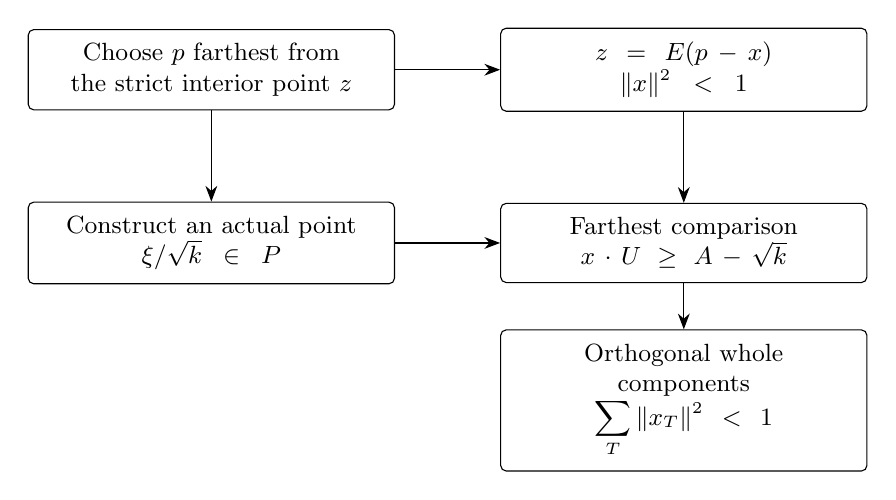
\begin{tikzpicture}[
 box/.style={draw,rounded corners=2pt,align=center,text width=43mm,
             inner sep=5pt,font=\small},
 >={Stealth[length=2mm]}]
\node[box] (far) at (0,2.8)
 {Choose \(p\) farthest from\\the strict interior point \(z\)};
\node[box] (vec) at (6,2.8)
 {\(z=E(p-x)\)\\\(\|x\|^2<1\)};
\node[box] (actual) at (0,.6)
 {Construct an actual point\\\(\xi/\sqrt k\in P\)};
\node[box] (pressure) at (6,.6)
 {Farthest comparison\\\(x\cdot U\ge A-\sqrt k\)};
\node[box] (budget) at (6,-1.4)
 {Orthogonal whole components\\
  \(\displaystyle\sum_T\|x_T\|^2<1\)};
\draw[->] (far)--(vec);
\draw[->] (far)--(actual);
\draw[->] (actual)--(pressure);
\draw[->] (vec)--(pressure);
\draw[->] (pressure)--(budget);
\end{tikzpicture}
\caption{The common-vector argument. Every component cost is tested
on the same \(x\). Feasibility of the auxiliary point is proved
against all actual walls before its pressure is used.}
\label{fig:budget}
\end{figure}

\section{Finite-component costs and the two small debits}
\label{sec:ordinary}

We call a block ordinary when its actual energy is strictly greater
than its rank divided by $14$. The following internal estimates
provide the complete finite-type coverage needed later.

\begin{proposition}[Ordinary component interface]\label{prop:ordinary}
The bounds in Table~\ref{tab:ordinary} hold with arbitrary finite
spectators at a farthest vertex. There is at most one short $A_1$
direction, where short means $L<\operatorname{arsinh}(1/\sqrt2)$.
Every other $A_1$ pays more than $1/10$. Apart from that possible
direction, the only nonordinary small blocks are the two isolated
rank-two defects described below, each still paying more than $9/100$.
\end{proposition}

\begin{table}[ht]
\centering
\begin{tabular}{ll@{\qquad}ll}
\toprule
Type & Strict energy lower bound & Type & Strict energy lower bound\\
\midrule
$A_2$ & $319/2000$, with one exception &
$I_2(m),\,m\ge4$ & $1/7$, with one exception\\
$A_3,B_3,H_3$ & $1/4$ & $A_4$ & $2/7$\\
$B_4,D_4,F_4$ & $1/3$ & $H_4$ & $11/36$\\
$A_5$ & $3/8$ & $A_6$ & $3/7$\\
$B_5,B_6$ & $3/7$ & $B_7,B_8$ & $1/2,\ 4/7$\\
$D_5,D_6$ & $5/14,\ 3/7$ & $D_7,D_8$ & $1/2,\ 4/7$\\
$E_6,E_7,E_8$ & $9/20,\ 5/9,\ 2/3$ & &\\
\bottomrule
\end{tabular}
\caption{Internal ordinary rates. Every displayed nonexceptional
rate is at least rank$/14$, with a strict energy inequality.}
\label{tab:ordinary}
\end{table}

We prove the proposition in this section. The proofs use the common
geometry above and finite spherical classification; foreign components
are retained in every positive replacement. In the contact lists,
$m@j$ means contact $\cos(\pi/m)$ at old node $j$, and a missing
contact means zero. Put $h=A^2$, and write the own and total foreign
costs of a wall as $q$ and $Q$, so that $h=q+Q-1>0$.

\begin{lemma}[Common-wall forcing and isolation]\label{lem:ordinaryforcing}
Suppose the energy of a component is at most $e$. A pair for which
the right side of \eqref{eq:pairupper} is below $K_{ij}$ has one
actual opposite. If one wall closes every direction of the component,
then, with $v_i=(C\beta)_i/\sqrt{d_i}$ and
$R_e^2=4e/(1+e)^2$,
\begin{equation}\label{eq:commoncost}
 q-1\le h\le R_e^2\min_i v_i^2.
\end{equation}
If $h<1/4$, it has no foreign contact. In a path, a wall closing
every direction can have multiple contacts only at the two endpoints;
in a $D_4$ star it has at most one.
\end{lemma}
\begin{proof}
The first assertion is \eqref{eq:pairupper}. For a closed direction,
$\tanh L_i=A/v_i$ and $\tau_i^2\le e$, which gives
\eqref{eq:commoncost}. Every nonzero foreign cost is at least $1/4$
and is strictly below $h$ by \eqref{eq:foreign}; hence the isolation
assertion. If the old path between two contacts omits a direction
closed by the wall, deleting that direction leaves a cycle in an
actual finite replacement. This is impossible. The same argument
applies to every two contacts in a $D_4$ star. Finally, a single-contact
own cost $q=1$ gives an affine principal set, impossible even in the
presence of further spectators.
\end{proof}

\subsection{The short directions and their exact debits}

For a short $A_1$ opposite put $b=\beta^2$, $h=A^2$, and let $Q$
be its full foreign cost. Then
\[
 h=b+Q-1,\qquad h<b/3,\qquad Q<1-2b/3.
\]
Equation~\eqref{eq:foreign} rules out two foreign components.
With one, its cost must be the sole value below $1/3$, namely an
$A_1$ contact $3$ of cost $1/4$. Thus the only possibilities are
\[
 I:\ \hbox{isolated dotted }A_1,\quad 0<h<1/2;
 \qquad
 J:\ \hbox{dotted }A_1+A_{1,3},\quad 1/3<h<3/8.
\]
For completeness, with one foreign component,
$Q<h=b+Q-1$ forces $b>1$, and $Q<1/3$ then forces $Q=1/4$.
For $J$, the heavy edge contributes more than $A/2$ to
$x\cdot v$. The light shadow contributes at least
$A(1-\sqrt{1-1/(4h)})$; this is at least $A/2$ if $h\le1/3$.
Strict \eqref{eq:interior} therefore gives the asserted lower bound.
Native acuteness excludes two short walls. Indeed their height
product is below $1/2$, so their product must be zero. Disjoint
supports give a negative product, heavy overlaps give a spatial
product above $1/2$, and a sole light/light overlap of two $J$ walls
gives $1/4$, below their height product. None is zero. A $J$ heavy
direction has $\tanh^2L>4/13$, hence energy $>9/100$; its light
direction has $\tanh^2L>2/3>16/25$, hence energy $>1/4$.
Thus $J$ funds both $A_1$ factors above their combined ordinary
baseline $2/10$. Every nonshort direction pays at least
$5-2\sqrt6>1/10$, since $\sqrt6<49/20$. We may conservatively
discard the one short direction, but only the isolated type $I$
can create an unfunded debit.

The rank-two exceptions are
\begin{equation}\label{eq:defects}
\begin{array}{c|c|c}
\hbox{old block / new isolated contact} & h=A^2 & \hbox{energy}\\ \hline
A_2/7 & (4/3)\cos^2(\pi/7)-1\in(0,1/12) & >9/100\\
I_2(7)/3 & (1/4)\csc^2(\pi/7)-1\in(0,1/3) & >9/100.
\end{array}
\end{equation}
Their spatial supports lie entirely in their own blocks.
Two defects in different blocks, or a defect and a short $A_1$,
would have actual wall product $-\sqrt{h_1h_2}\in(-1/2,0)$.
That interval is forbidden: distinct acute unit walls have product
$0$ or at most $-1/2$. Therefore
\begin{equation}\label{eq:debits}
\text{at most one short }A_1,\quad\hbox{or one rank-two defect,
but never both.}
\end{equation}
This argument is independent of every other component type.

\subsection{The two rank-two estimates}

For $A_2$, set $e_2=319/2000$ and $\sinh^2L_0=31/50$.
If both edges have length at least $L_0$, then their half-tangents
exceed $173/500$ and energy is greater than
$4\cdot173^2/(3\cdot500^2)>e_2$. A shorter edge cannot have two
positive own contacts: $3/3$ is affine, while $3/4$ or larger gives
$\sinh^2L\ge4\sqrt2/9>31/50$, increasing with either contact
and with $Q$. If only the other node is contacted, apply the same
test to that shorter contacted direction. For one contact of square
$b$, the shorter-edge condition is
\begin{equation}\label{eq:A2short}
 h=4b/3+Q-1<124b/243,\qquad Q<1-200b/243.
\end{equation}
Every positive foreign cost must be below $h$. A label $3$ gives
$h<1/4$, hence isolation and negative height. For a label $4$,
$h<62/243$ forces each foreign cost to be $1/4$; the only positive
possibility is $Q=1/2$, but then $h=1/6<1/4$. A label $5$ has
$Q<1/2$, hence at most one foreign component, whose cost exceeds
$h$ because its own cost $\ph^2/3$ is below one. A label $6$ is
affine. For a finite label $m\ge7$, $b>.81$ gives $Q<1/3$;
thus $Q=0$ or $Q=1/4$. The latter is possible in
\eqref{eq:A2short} only for $b<729/800$, namely $m=7,8,9,10$.
Indeed $\cos^2(\pi/11)>45/49>729/800$, using $\pi<22/7$.
A dotted contact has $Q<1/4$ and is isolated.

For an isolated finite contact the same wall closes the mate,
since its reciprocal ratio squared is $b/(4b-3)>1$.
For $m\ge8$ that actual mate has
$\tanh^2L\ge6\sqrt2-8>400/841$, so its energy exceeds
$4/25>e_2$. For an isolated dotted contact,
$b<243/200$ and its distinct mate has shadow
$\tanh^2L\ge b/(4b-3)>81/124>16/25$.
For a mixed $m=7,8,9,10$ contact, the mate's white cost is
$b+1/4>1$; the distinct shadow instead gives
$\tanh^2L\ge b/(4b-9/4)>11/17>16/25$.
Both give energy greater than $1/4$. Thus the only exception is
isolated new $7$ at old $A_2$.
The root $t=\cos(2\pi/7)$ of $8t^3+4t^2-4t-1$ lies in
$(623/1000,5/8)$: the polynomial changes sign there and is increasing
on $[1/2,1]$. Hence $b>1623/2000$ and its actual mate satisfies
$\tanh^2L=4-3/b>164/541>3600/11881$, proving its cost $>9/100$.

For an old $I_2(m)$, $m\ge4$, put $k=\cos(\pi/m)$ and
$d=(1-k^2)^{-1}$, so $C=d\left(\begin{smallmatrix}1&k\\k&1\end{smallmatrix}\right)$.
At energy at most $1/7$, \eqref{eq:pairupper} forces one common
opposite. Two contacts give an actual
$\cosh L\ge\cot(\pi/(2m))/\sqrt3>11/8$, with individual energy
$>3/19>1/7$. For one contact $\beta$,
\begin{equation}\label{eq:dihedralcut}
 q(1-7k^2/16)\le1,\qquad q=d\beta^2.
\end{equation}
Its minimum left side is $(9d+7)/64$. Since
$m\ge8$ gives $d\ge4+2\sqrt2>19/3$, only four old labels remain:
\[
\begin{array}{c|l}
m&\text{consequence of \eqref{eq:dihedralcut}}\\ \hline
4&\beta^2\le16/25<\cos^2(\pi/5):\ 3,4;\ h\le7/32<1/4,\ q\le1;\\
5&d>25/9:\ \text{only }3;\ h<7/32,\ q<1;\\
6&\text{only }3;\ q=1;\\
7&d>5:\ \text{only }3;\ Q<3/16.
\end{array}
\]
Isolation or the affine principal excludes the first three rows.
The last is isolated new $3$ at old $I_2(7)$, with $0<h<1/3$.
Its actual mate has $\cosh L=\cot(\pi/7)/\sqrt3>109/91$ by the
same cubic bracket; the squared comparison has positive numerator
$2652$. Thus its energy also exceeds $9/100$, completing
\eqref{eq:defects} and \eqref{eq:debits}.

\subsection{Rank three and four: one common-wall calculation}

For energy $1/4$, adjacent correlation at least $1/\sqrt3$ forces
a common opposite: the lowest cleared comparison is
$74/\sqrt3>39$. At energy $1/3$ the threshold $1/\sqrt2$ works,
since $51/\sqrt2>34$. For $A_4$ at energy $2/7$, the adjacent
correlations are $\sqrt{3/8},2/3,\sqrt{3/8}$; the forcing test is
$k^3+16k^2+36k-28>0$, whose lowest value is positive because
$291\sqrt6>704$. Direct inversion verifies the indicated
correlation thresholds for $A_3,B_3,H_3$ and $B_4,D_4,F_4$.
For $H_4$ use energy $11/36<1/3$. Thus a common wall closes all
directions in every case.

Number path bonds as $A_3:(3,3)$, $B_3:(4,3)$, $H_3:(5,3)$,
$A_4:(3,3,3)$, $B_4:(4,3,3)$, $F_4:(3,4,3)$, and
$H_4:(5,3,3)$. By Lemma~\ref{lem:ordinaryforcing}, multiple
contacts can only be at the endpoints. Two endpoint $3$ contacts
in $A_3,A_4$ are affine; the next minimum is $3/4$. In the other
rows below even $3/3$ is excluded. The displayed values are lower
bounds for $q-R_e^2v_j^2$, contradicting \eqref{eq:commoncost}:
\[
\begin{array}{c|c|c}
T&j&\text{lower bound}\\ \hline
A_3&2&177/200+9\sqrt2/100>1\\
A_4&2&(230+15\sqrt2)/243>1\\
B_3&2&(77+18\sqrt2)/100>1\\
B_4&3&15/16+\sqrt2/8>1\\
F_4&2&15/16+\sqrt2/4>1\\
H_3&2&(72\ph+95)/100>1.
\end{array}
\]
$D_4$ already has at most one contact. In $H_4$, two endpoint
contacts retain, after deleting old node $4$, a path at least
$(3,5,3)$ of determinant $(5-4\ph)/16<0$. Hence all contacts
are single.

For a single contact at $j$ let
$\sigma_j=\min_i(v_i^2/q)$. Formula \eqref{eq:commoncost} gives
$q\le(1-R_e^2\sigma_j)^{-1}$. The complete inverse calculation
is as follows; entries are in path order, and $D_4$ means leaf,center.
\begin{center}\small
\begin{tabular}{ccll}
\toprule
$T$&$d_j$&$\sigma_j$&upper $q$\\ \midrule
$A_3$&$3/2,2,3/2$&$1/9,1/3,1/9$&$225/209,75/59,225/209$\\
$A_4$&$8/5,12/5,12/5,8/5$&$1/16,1/6,1/6,1/16$&$162/155,243/215,243/215,162/155$\\
$B_3$&$3,4,2$&$1/3,1/2,1/3$&$75/59,25/17,75/59$\\
$D_4$&$2,4$&$1/4,1/2$&$16/13,8/5$\\
$B_4$&$4,6,4,2$&$1/4,1/3,1/2,1/4$&$16/13,4/3,8/5,16/13$\\
$F_4$&$4,12,12,4$&$1/2,2/3,2/3,1/2$&$8/5,2,2,8/5$\\ \bottomrule
\end{tabular}\end{center}
Here $R_e^2$ is respectively $16/25$, $56/81$ for $A_4$, and
$3/4$ for the $1/3$ rows. Dividing the upper $q$ by $d_j$
gives the finite native lists:
$A_3$ endpoints $3/4/5$, middle $3/4$;
$A_4$ endpoints $3/4$, inner $3$;
$B_3$ nodes $3;3;3/4$;
$D_4$ leaf $3/4$, center $3$;
$B_4$ nodes $3;\varnothing;3;3/4$;
$F_4$ endpoints $3$, inner $\varnothing$.
Each has $q\le1$. Equality is affine; in every other listed case
\eqref{eq:commoncost} gives $h<1/4$ (the largest needed bounds are
$16/75,7/155,28/405,3/16$). Isolation then gives $h=q-1<0$.
This proves the six crystallographic and $A$ rows.

For $H_3$, the minimum contact $\beta=1/2$ at node $1$ or $2$
gives tests at node $3$ equal to
$(199\ph+263)/500$ and $(61\ph+77)/125$, both above one.
At node $3$, $\beta\ge1/\sqrt2$ gives the test at node $1$
at least $(27\ph+118)/150>1$. Only $3@3$ remains, with
$q=(\ph+2)/4<1$ and $h\le4\ph^4/75<\ph/4$.
No spectator gives negative height; one has cost $Q>h$; two have
$Q\ge1/2$ and hence $h\ge q-1/2=\ph/4$. All are impossible.
For $H_4$, $R_e^2=1584/2209$; at $\beta=1/2$ the four tests
(contact node, test direction) are
\[
(1,4):\frac{4938\ph+3688}{2209},\quad
(2,4):\frac{7209\ph+5334}{2209},\quad
(3,1):\frac{2500\ph+2667}{2209},\quad
(4,1):\frac{625\ph+1219}{2209}.
\]
All exceed one, the last by $\ph>198/125$; larger contacts only
increase these positive tests. This proves $H_4>11/36$.

\subsection{The two intermediate \texorpdfstring{$A$}{A} components}

Use $C_{ij}=2\min(i,j)(N-\max(i,j))/N$, with $N=6,7$.
For $A_5$, distinct $2/3$ and $3/4$ pairs each demand a sum above
$109/100$. The vector $u_2+2u_3+u_4$ has square
$7+4\sqrt2<443/35$, and
\[
(109/50)^2-(3/8)(443/35)=209/35000>0.
\]
For $A_6$, the three pair demands are
\[
2249/2000,\qquad11547/10000,\qquad2249/2000;
\]
the vector $u_2+2u_3+2u_4+u_5$ has square
$<33781/1250$, with demand $34037/10000$ and Cauchy gap
$2181583/700000000$ at energy $3/7$.
These pair bounds follow by substitution in
$F(s/2)^2<K$. Thus a common $2/3$ occurs for $A_5$, and a common
$2/3$ or $3/4$ for $A_6$, up to reversal.

Each retained path allows one contact. The full two-contact list is
\begin{center}\small
\begin{tabular}{lll}
\toprule
Component/pair&positions&necessary finite-white labels\\ \midrule
$A_5,2/3$&$1,3$&$3/3$ or $4@1+3@3$\\
&$1,4;1,5;2,4;2,5$&both $3$\\
&$2,3$&both in $3,4,5$\\
$A_6,2/3$&$1,3$&$3/3$ or $4@1+3@3$\\
&$1,4;1,5;1,6;2,4;2,5;2,6$&both $3$\\
&$2,3$&$3,4,5$ at $2$; $3,4$ at $3$\\
$A_6,3/4$&$3,4$&both in $3,4,5$\\
&other eight left/right pairs&both $3$\\ \bottomrule
\end{tabular}\end{center}
Indeed deletion of either closed node leaves a connected finite
path or $D/E_6$ tree: a $4$ can only be terminal, and $D/E$ bonds
are all $3$. All-$3$ doubles are affine cycles. The adjacent
non-$3/3$ doubles force an actual edge of cosh at least
$(3+\sqrt2)/2>11/5$ in $A_5$; for $A_6$ the minimum formulas are
$(5+4\sqrt2)/\sqrt7$, $(4\sqrt2+6)/\sqrt{14}$, and
$(12+9\sqrt2)/\sqrt{42}$, all above $5/2$.
The $A_5$ terminal-$4$ row has $Q=0$ and cosh
$(3+\sqrt2)/2$. The $A_6$ version has white cost $9/10$, hence
$Q=0$, and is treated below. These cosh thresholds imply individual
energies above $3/8$ and $3/7$.

For single $3$ contacts the complete own costs and strict white
bounds are
\[
\begin{array}{c|c|c|c}
\text{component/pair}&j&q&Q\text{ upper}\\ \hline
A_5,2/3&1,2,3,4,5&5/12,2/3,3/4,2/3,5/12&2/3,2/3,5/8,1/2,5/8\\
A_6,2/3&1,2,3,4,5,6&3/7,5/7,6/7,6/7,5/7,3/7&2/3,2/3,3/5,2/5,2/5,3/5\\
A_6,3/4&1/6;2/5;3/4&3/7;5/7;6/7&5/8;1/2;5/8.
\end{array}
\]
End and small-$Q$ rows have $h<1/4$, or only one foreign
component with cost $Q>h$. In $A_5$ at $j=2,3$ two foreign
components would each exceed $1/3,1/4$, respectively, forcing
$Q\ge2/3$; the same gap treats $A_6,j=2$.
In the remaining $A_6,j=3,4$ rows, two foreign bonds must be $3$
since $Q<5/8$; together with the contacted old node and its two
neighbors they form affine two-fork $D_5$. This excludes all single
$3$ cases. A single internal $4$ gives the affine $(3,3,4)$ star;
an end $4$ has $Q\le1/3$ and $h<1/4$, again impossible.

A single $5$ is at a retained path end; its $H_3/H_4$ white cost
exceeds $3/4$, so $Q=0$. All cases are covered by these actual
positive replacements:
\[
\begin{array}{c|c|c|c}
\text{component/pair}&\text{contact}&\text{actual direction}&\cosh L\\ \hline
A_5,2/3&1\text{ or }5&4\text{ or }2&\ph^3/\sqrt3\\
&2&3&\ph^2\\
&3&2&\sqrt3\ph^3\\
A_6,2/3&1&4&3\ph^3/\sqrt{21}\\
&2&3&4\ph^2/\sqrt{14}\\
A_6,3/4&1\text{ or }6&4\text{ or }3&3\ph^3/\sqrt{21}\\
&3\text{ or }4&4\text{ or }3&9\ph^3/\sqrt{21}.
\end{array}
\]
The first group exceeds $11/5$, the second $5/2$, using
$\ph>8/5$, $\sqrt{21}<23/5$, $\sqrt{14}<15/4$.
No new wall is inferred: each replacement contains the already
actual $c$. Finally the $A_6$ double $4@1+3@3$ has the positive
actual future point
\[
 \xi=c+(\sqrt2-1/2)n_1+(\sqrt2-1)n_2+(\sqrt2/2)n_3,
 \qquad \xi^2=5/4-\sqrt2=-k.
\]
Its products with $c,n_1,n_3$ vanish and its product with $n_2$
is $(\sqrt2-3)/4<0$. Here $A^2=(5+4\sqrt2)/7$ and
$A^2-9k=(335-236\sqrt2)/28>0$; \eqref{eq:pointenergy} gives
energy $>(A-\sqrt k)/(A+\sqrt k)>1/2$.

\subsection{The four intermediate \texorpdfstring{$B$}{B} components}

Use $u_i=(e_1+\cdots+e_i)/\sqrt i$ and, for $i<r$,
$\omega_i=\sqrt2(e_1+\cdots+e_i)$, while
$\omega_r=e_1+\cdots+e_r$.
At energies $3/7,1/2,4/7$ the relevant forcing signs are
$127\sqrt{2/3}-100$, $(69\sqrt{6/7}-52)/7$, and
$(199\sqrt{6/7}-176)/7$, all positive.
Thus $B_5,B_6$ have a common $2/3$, and $B_7,B_8$ a common $6/7$.

For $B_5,B_6$, deletion $2$ retains $A_1+B_3/B_4$.
The right contact is $3@3$, with the sole $B_5$ exception $3@5$
giving $F_4$; deletion $3$ allows one left $3/4/5$.
For $3@3$, own $0$ is affine, own $3$ is a triangle, and own
$\ge4$ gives $\cosh L_3\ge2+3/\sqrt2>3$.
With no right contact the complete choices are $3/4/5$ at $1$ or
$2$: $3@2$ and either $4$ are affine; $3@1$ has
$h=Q-1/2<1/6$ and closes a forbidden foreign direction.
The two $5$ cases have $Q=0$: $5@1$ also closes $4$ with
$\cosh L_4=\ph^3>3$, and $5@2$ has
$\cosh^2L_3=2\ph^2/(2-\ph)>9$.
For the $B_5$ short-end $3@5$, finite $F_4$ forbids left $1$
and all spectators; own $0$ is affine and the other replacement
forces own $3$, giving $\cosh L_2=2+\sqrt2$.
Every branch exceeds the individual threshold $11/5$.

For the $6/7$ pair, a wall without a right contact has a single
left $3$ or endpoint $4$. Apart from far $3@1$ these give an
affine fork, double-$4$, or star. A minimal nonpositive principal
for the far branch must contain $c,7$, since deletion $7$ is
finite; their connecting path $c,1,\ldots,7$ has eight vertices.
Spectators attach through $c$ and do not shorten it. This violates
the Lann\'er order bound, excluding the branch with all spectators.
In $B_7$, let $\beta$ be the contact to the retained right $A_1$:
\[
\begin{array}{c|l|l}
\beta/\text{own }6&\text{left contacts}&\text{pressure or rejection}\\ \hline
\beta\ge\cos(\pi/5),\ \text{any}&\text{none}&\cosh L_6\ge\sqrt6\cot(\pi/5)>3\\
\beta_4,0&\text{any allowed}&\text{affine }(4,4)\\
\beta_4,>0&\text{none}&\cosh L_6\ge\sqrt{24}\\
\beta_3,>0&\text{none}&\cosh L_6\ge2+\sqrt2\\
\beta_3,0&\text{none or }1&\text{affine }F_4\\
\beta_3,0&\text{one }j=2,\ldots,5&\cosh L_6\ge1+3/\sqrt2>3.
\end{array}
\]
Here $\beta_m=\cos(\pi/m)$. The last row retains the full foreign
cost: its white residual is
$\Delta\le3/4-j(6-j)/12\le1/3$, and
$v_6\ge\sqrt{12}(j/12+1/(2\sqrt2))$.
Thus no allowed $E_7$ extension is silently removed.

In $B_8$ the retained right $B_2$ has one simple $3$ at either
end. At long end $7$, own $0/3$ is affine and own $4$ gives
$\cosh L_7\ge6+7/\sqrt2>7$.
At short end $8$, own $>0$ gives
$\cosh L_6\ge\sqrt6+\sqrt3>11/3$.
At own $0$, the left-white budget permits only $3@1$ or $3@5$:
none or $1$ gives affine $F_4$, but $3@5$ is an allowed bridge,
with $\Delta\le1/12$ and
$v_6=\sqrt{12}(5/12+1/(2\sqrt2))$.
It has $\cosh L_6\ge5+3\sqrt2>9$; it is estimated, not removed
by an incorrect $F_4$ sealing claim. These complete lists prove
the four asserted $B$ costs.

\subsection{Extended stars, \texorpdfstring{$D_7$}{D7}, and the \texorpdfstring{$D_8$}{D8} closure}

Let $S$ be a central $D_4$ star with an extended arm. If one wall
closes its center and three neighbors, every minimal nonpositive
principal contains $c$ and all four nodes of $S$, since deletion
of any of them is an actual finite replacement. Compactness and
the Lann\'er order bound make that principal exactly $S+c$.
Two contacts give a nonpositive proper triangle or cycle.
A sole center $3$ is affine, and a larger center contact has a
nonpositive proper star. A sole leaf contact is $3/4/5$ from its
finite proper path: $3$ gives finite $D_5$, $4$ affine, leaving
only $5$. If that leaf extends, it retains a nonpositive $(5,3,3)$
star; if another arm extends, it retains a nonpositive $(5,3,3,3)$
path. Each omits a supposedly closed $S$ direction, a contradiction.
Further negative contacts cannot repair the positive nonpositive
quadratic witness. Thus the four opposites cannot all coincide.

For $D_5,D_6$ the minimum central correlations are
$\sqrt{3/5},\sqrt{2/3}$. At energies $5/14,3/7$ the forcing
signs are $544\sqrt{3/5}-362$ and $127\sqrt{2/3}-100$, positive.
For $E_6,E_7,E_8$ the arm lengths are $(1,2,L)$ with $L=2,3,4$.
In raw norm-two coordinates the central Schur residual is
$\delta=2-[1/2+2/3+L/(L+1)]$; on an arm of length $m$, squared
central correlation is $t/(\delta+t)$, $t=m/(m+1)$.
The minima are $\sqrt3/2,\sqrt{6/7},\sqrt{15}/4$.
At energies $9/20,5/9,2/3$ even $4e/(1+e)^2$ lies below these
correlations. All four opposites would coincide, proving the five
extended-star costs.

For $D_7$ write $o=r-2$, $a=r-3$, with fork leaves $b,f$.
At energy at most $1/2$, correlation $\sqrt{4/5}$ forces a
common $o,a$. Deletion $a$ retains $A_3=b-o-f$, so its right
contact is none, middle $3$, or endpoint $3/4/5$; deletion $o$
allows one left contact. The complete surviving profiles are
\begin{equation}\label{eq:D7roles}
 4@a+3@o,\qquad\text{isolated }5@b,\qquad3@a+4@b,
\end{equation}
up to exchanging the fork leaves. To check the list: middle $3$
forces $4@a$ (own $0/3$ is affine); endpoint $5$ seals all white
extensions by $H_4$, and a contact at the removed $a$ leaves a
nonpositive $(3,3,3,5)$ path. Endpoint $4$ forces $3@a$, otherwise
an affine terminal-$4$ fork remains. Endpoint $3$ excludes every
left contact by cycles or retained $F_4$; a foreign $3$ is affine
$E_7$, a foreign $4$ is an affine terminal-$4$ fork, and larger
foreign bonds are nonfinite. Its isolated height is negative for
$r=7$ and it contains affine $E_8$ for $r\ge8$.
With no right contact, internal-left $3$ and endpoint $4$ are
affine; far-left $3$ needs a Lann\'er path of at least six vertices.
This accounts for all spectators as well as the removed own contact.
The first and third roles have
$\cosh L_o=a+(r-2)/\sqrt2>7$.
The isolated $5$ has
$\tanh^2L_a=1-(9-4\sqrt5)/(r-3)$; at $r=7$ its half-tangent
square is $4/\sqrt5-1>3/4$. Each role therefore contradicts
energy at most $1/2$, proving the $D_7$ cost.

For $D_8$, common $4/5$ has exactly $4@4+3@5$.
Indeed deletion $4$ permits simple $3$ at a right $D_4$ leaf,
and deletion $5$ allows one left $3$ or endpoint $4$.
Long-leaf $3$ forces $4@4$ and forbids foreign contacts by the
retained $(3,4,3,3)$ path. A fork $3$ with a left $3$ gives an
affine cycle; without a left contact it is affine $E_8$; a left
$4$ is nonpositive. With no right contact only far $3@1$ survives
the affine tests, but its path to $5$ has six vertices.
Common $5/6$ has the preceding center-neighbor list. Both common
pairs thus force an actual half-tangent square above $3/4$.
At energy at most $4/7$, their opposites are distinct.

Here is the remaining three-direction calculation. Put
$q=\sqrt{4/5}$, $k=\sqrt{5/6}$, $\lambda=(1+k)/2$,
$\alpha=k\sqrt{1-k}/2$, $e=4/7$, and
$P(t)=t/(1+\sqrt{1-t})^2$.
Write $h_i=x\cdot u_i$ and decompose
$x=aw+bv+zt_0+y$, where $w,v$ are the normalized sum and
difference of $u_5,u_6$, $u_4=qu_5+t_0/\sqrt5$, and
$y\perp w,v,t_0$. The full-tangent laws imply
\[
 h_4h_5\ge P(q),\qquad
 T:=(1+\alpha)b^2+\lambda z^2
 \le\delta:=\lambda e-P(k)<1/400.
\]
For the second inequality take the tangent line to
$4p/k-(1+p)^2$ at its first zero $p=P(k)$, with
$p=h_5h_6=\lambda a^2-(1-\lambda)b^2$.
Keeping the negative quadratic terms in $h_4h_5$ gives
\[
 h_4h_5\le q\lambda e+A_0|b|+B_0|z|
              -qkb^2-q\lambda z^2,\qquad
 A_0^2=8/105,\quad B_0^2=4/35.
\]
Weighted Cauchy bounds the linear part by $\sqrt{C_0T}$, where
$C_0=(8/105)/(1+\alpha)+(4/35)/\lambda<47/250$.
Also $qk/(1+\alpha)>.71$, $q>.71$, and $q\lambda e<.489$.
Consequently
\[
 h_4h_5<.489+\sqrt{(47/250)T}-.71T
 <101781/200000<.509<P(q),
\]
a contradiction. The rational seals are
$.8944<q<.8945$, $.9128<k<.9129$,
$.29<\sqrt{1-k}<.2953$, $.13<\alpha<.14$,
and $.95<\lambda<.95645$.
The tight $\delta$ comparison reduces to
$91280000\cdot70000-167780209\cdot38083=26300653>0$;
the last square-root comparison uses
$\sqrt{47/100000}<271/12500$.
This proves $D_8>4/7$ and completes Proposition~\ref{prop:ordinary}.

\section{Two classical interfaces used in the composition}
\label{sec:interfaces}

\begin{proposition}[Actual $B/D$ floor]\label{prop:BDnine}
Every whole $B_r$ or $D_r$ component with $r\ge9$ has actual
projection energy greater than $9/14$, with arbitrary finite
spectators.
\end{proposition}

\begin{proof}
Assume energy at most $e=9/14$. In $B$ it suffices to bound the first
seven coordinates; all displacements below lie there. The normalized
directions in either type are $u_i=(e_1+\cdots+e_i)/\sqrt i$.
We first establish distinctness of $4/5,6/7$, then use those laws to
exclude all common $1/2,2/3$ profiles. This order is noncircular.

For an internal common $i/(i+1)$ with right retained rank at least
four, finite classification permits a right long-leaf $3$, or none.
The first forces own $4$: own $0/3$ is affine fork/triangle, and
any foreign contact retains the nonpositive $(3,4,3,3)$ path.
Without a right contact, internal-left $3$ and endpoint $4$ are
affine. Only far $3@1$ remains, but its path to $i+1$ has at least
six vertices, contradicting the Lann\'er bound. Right $D$-fork
contacts give affine $E_8$ or a cycle with the left contact.
Thus the sole common profile is $4@i+3@(i+1)$, $Q=0$, with
$\cosh L_{i+1}=i+(i+1)/\sqrt2>7$.
The $D_8$ right-$D_4$ and center-neighbor boundary calculations are
in Section~\ref{sec:ordinary}; the center-neighbor calculation also
handles $D_9$ at $6/7$.
In $B_9$, the extra right short-end $3@9$ gives $F_4$, excluding
left and foreign white contacts. The removed own $6$ remains to check:
own $0$ is affine $F_4$, own $4$ the affine $(4,3,3)$ star, and own
$3$ gives $\cosh L_6=(1+1/\sqrt2)\sqrt{12}>11/2$ and
$\tau_6^2>9/13>e$. Consequently $4/5$ and $6/7$ are distinct.

Write $h_i=x\cdot u_i$. Distinct $6/7$ gives
$h_6h_7\ge k/(1+\sqrt{1-k})^2>9/16$, where
$k=\sqrt{6/7}>576/625$ with squared margin $21318$.
Hence $x\cdot w>3/2$ for $w=u_6+u_7$.
We record four local tests with their exact margins.

\emph{Edge $2$ with $\cosh L_2\ge1+\sqrt2$.}
Then $h_2^2\ge\sqrt2-1$. Projection of $w$ about $u_2$ has
$\rho=1/\sqrt3+\sqrt{2/7}<1.114$ and residual square
$S=29/21+4\sqrt{2/21}<2.62$.
Its Cauchy envelope $\rho t+\sqrt{S(e-t^2)}$ decreases for
$t\ge q=\sqrt{\sqrt2-1}$: its derivative condition follows from
$\rho^2e<13/16<6/5<\|w\|^2q^2$.
Since $q<.644$, $e-q^2<.23$, and $\sqrt{2.62\cdot.23}<.777$,
$x\cdot w<1.114(.644)+.777=1.494416<3/2$.
These follow by squaring, using $1.414<\sqrt2<1.4143$,
$1/\sqrt3<.578$, $\sqrt{2/7}<.535$, $\sqrt{2/21}<.309$.

\emph{Isolated $5@1$.}
Its height square is $(\ph-1)/2$ and its actual direction-$4$
shadow has $\tau_4^2=\ph-1$. For the same $w$, projection about
$u_4$ has $\rho=2(1/\sqrt6+1/\sqrt7)<787/500$ and
$S=16/21+4/\sqrt{42}<69/50$. Use
$1/\sqrt6<.409$, $1/\sqrt7<.378$, $\sqrt{42}>162/25$;
the last residual comparison has cleared margin $23$.
Since $\sqrt e<401/500$, $e-(\ph-1)<1/40$ and
$(93/500)^2>69/2000$, Cauchy gives
$x\cdot w<362087/250000<3/2$.

\emph{Isolated $5@2$.}
Its height square is $\ph$. The direction-$1$ shadow gives
$x_1>31/50$, since $F(31/50)^2<161/200<\ph/2$ with cleared
margin $6541881$. Its actual edge $3$ has
$\cosh L_3=\sqrt2\ph^2>37/10$; hence
$S_3=x_1+x_2+x_3>131/100$, using
$3\tau_3^2>81/47>(131/100)^2$, of margin $3433$.
Distinct $4/5$ gives $x\cdot w_0>57/40$, $w_0=u_4+u_5$.
Put $v=e_1+e_2+e_3$, $k_0=1/2+1/\sqrt5<237/250$, and
$x_0=(31/50,69/200,69/200,0,\ldots)$.
Then $x_0=(11/40)e_1+(69/200)v$, $x\cdot x_0>x_0^2>31/50$.
The residual $w_0-k_0v$ has square $13/20+1/\sqrt5<11/10$
and excess demand $>9/50$.
All coefficients of $x_0+(w_0-k_0v)/6$ remain positive, and its
Cauchy margin is at least
\[
 (31/50+(9/50)/6)^2-e(31/50+(11/10)/36)=3/700>0.
\]

\emph{Contacts $4@2+3@3$.}
The white $A_2$ cost is $2/3$, so $Q=0$ or $1/4$; the latter has
$\cosh L_3=4+3\sqrt2>7$. At $Q=0$, put $s=\sqrt2$.
The actual floors satisfy
$\tau_2^2=(1+2s)/7$, $\tau_3^2=(2s-1)/3$,
$\tau_2\tau_3=1/\sqrt3$.
Their positive equality vector has $E_0=(6s-4)/7>.6407$.
The positive old-$A_2$ correction of $c$ is an actual future point
of square $-s/3$, giving pure displacement
\[
 U=\frac{2+s}{2}e_1+\frac{1+s}{3}(e_2+e_3+e_4),\qquad
 x\cdot U\ge A-\sqrt{s/3},\quad A^2=(5+4s)/2.
\]
Its projection coefficients on $u_2,u_3$ are
$\rho_2=(2s+1)/6$, $\rho_3=(1+s)/\sqrt3$;
its residual square is $(7+4s)/12<1.055$, with excess demand
$\Delta>.06$.
Indeed $1.4142<s<1.4143$ gives $A>2.3083$,
$\sqrt{s/3}<.6867$, $\tau_2\in(.7395,.7396)$,
$\tau_3\in(.7806,.7808)$, $\rho_2<.6381$, $\rho_3<1.394$,
and excess $>.06122604$.
The old positive coefficients exceed $.3,.52$; subtracting
$(\rho_2,\rho_3)/16$ removes less than $.04,.088$.
The corrected dual therefore has Cauchy margin at least
\[
 (.6407+.06/16)^2-e(.6407+1.055/256)
       =8825113/11200000000>0.
\]
This is an actual-point constraint, not an edge-only assertion.

Now exhaust common $1/2$. Deletion $1$ retains right rank at least
eight, so the right contact is none or long-leaf $3@2$.
The latter forces own $\gamma\ge1/\sqrt2$ (own $0/3$ is affine),
and $\cosh L_2=(1+\gamma)/\sqrt{1-\gamma^2-Q}\ge1+\sqrt2$,
already excluded. Without a right contact,
$A^2=2\gamma^2+Q-1>0$ and $\gamma^2+Q<1$.
Own $0$ has zero derivative; own $3$ has height below $1/4$ and
forces a foreign closure; own $4/6$ is affine.
Own $5$ with $Q>0$ has $\cosh L_2\ge\ph^2>1+\sqrt2$;
at $Q=0$ use the isolated-$5$ test. Finite $m\ge7$ forces $Q=0$;
$m\ge8$ uses the edge-$2$ test, leaving only isolated $7$.

For common $2/3$, deletion $2$ retains right $B/D$ rank at least
seven; deletion $3$ allows one left $3/4/5$ at $1$ or $2$.
A right long $3@3$ forces own $3/4/5$: own $0$ is affine, own $3$
a triangle, own $4$ is the tested $4+3$ profile, and own $5$ has
$Q=0$, $\cosh L_3=(2+5\ph)/\sqrt2>7$.
Without a right contact the full left list is
$3@1,4@1,5@1,3@2,4@2,5@2$.
The first has $A^2=Q-1/2<1/6$ and forces foreign closure;
$4@1,3@2,4@2$ are respectively affine terminal-$4$, two-fork,
and $(4,3,3)$ star. The $5$ cases have $Q=0$ by white cost
$\ph^2/3>3/4$ and were tested above.
For $D_9$ one extra right-fork $3$ gives retained $D_7+c=E_8$.
It excludes old-$1$ and foreign contacts, but the removed own $2$
must still be checked: own $0/3/4$ gives affine $E_8$/cycle/star,
and own $5$ retains nonpositive $(3,5,3)$. At higher rank the fork
attachment already contains affine $E_8$. No finite branch is omitted.

For the final isolated $7@1$, put $t=\cos(2\pi/7)$,
$g=\cos(\pi/7)$, and
\[
 \xi=c+g^{-1}n_1+(1-t)g^{-1}n_2
     =\sqrt t\,p-\frac V{\sqrt{1+t}},\qquad
 V=t(e_1+e_2)+(1-t)e_3.
\]
It has $\xi\cdot c=\xi\cdot n_1=0$,
$\xi\cdot n_2=(1/2-t)/g<0$ and
$\xi^2=-(1-t)(2t-1)/(1+t)<0$.
All coefficients and its time coefficient are positive, proving
actual feasibility and future orientation. Thus
$x\cdot V\ge\sqrt{t(1+t)}-\sqrt{(1-t)(2t-1)}$.
The increasing cubic $8t^3+4t^2-4t-1$ gives $.6234<t<.6235$,
with endpoint values $-.000926392768,.000105223$.
Hence the first radical is $>1.0059$, the second $<.305$,
and $.95<\|V\|<.9588<.959$, so $x\cdot\widehat V>.73$.
The projection of $w$ onto $\widehat V$ is
$\rho=(1/\sqrt6+1/\sqrt7)(1+t)/\|V\|\in(1.3,1.35)$,
and residual square is $<11/5$.
The Cauchy envelope decreases above $.73$, since
$\rho^2e<6561/5600<3(.73)^2<\|w\|^2(.73)^2$.
It gives $x\cdot w<1.35(.73)+.492=591/400<3/2$;
the final squared radical margin is $277/1750000$.
Thus $1/2,2/3,6/7$ all have distinct actual opposites.

Their exact pair sums are
\[
 x\cdot(u_1+u_2)>1.091,\quad
 x\cdot(u_2+u_3)>1.265,\quad
 x\cdot(u_6+u_7)>1.512.
\]
Set $W=.1(u_1+u_2)+.055(u_2+u_3)+.305(u_6+u_7)$. Direct positive
Gram estimates give
\[
\begin{gathered}
 x\cdot W>.639835,\qquad W^2<.636435825,\\
 .639835^2-\frac9{14}(.636435825)
 =\frac{70423123}{280000000000}>0.
\end{gathered}
\]
To verify the pair sums, use $F(a)F(b)\le F((a+b)/2)^2$.
The correlation lower bounds
\[
7071/10000,\qquad81649/100000,\qquad9258/10000
\]
have squared margins $959,\allowbreak322397,\allowbreak26052$ below the exact values.
At sums $m/1000$, $m=1091,\allowbreak1265,\allowbreak1512$, the cleared differences
\[
p(4000000+m^2)^2-16dm^2\,1000000
\]
are respectively
\[
40828209713231,\qquad358399613480625,\qquad52443946917888.
\]
The six upper Gram entries of the three pair vectors are
$3.415,3.633,3.852,3.102,1.899,2.474$, obtained by positive
squaring of their prefix correlations. Their expansion is the stated
bound on $W^2$. This contradicts Cauchy and proves the proposition.
\end{proof}

\begin{proposition}[Large-component caps]\label{prop:caps}
At a farthest vertex, with arbitrary finite spectators, the following
components are impossible:
\[
 A_r\ (21\le r\le29),\qquad B_r\ (23\le r\le29),\qquad
 D_r\ (24\le r\le29).
\]
\end{proposition}

These are internal theorems. We give their finite continuation and
energy proofs below. All references to old directions concern the
chosen farthest vertex, and all added walls are already actual.

\subsection{Clearing spectators and the finite continuation list}
\label{sec:capinventory}

Put $c_0=61/100$. For a long index, write $D_i=\omega_i^2$,
$q_i=\sqrt{D_i}$ and $h_i=x\cdot\omega_i$, and call it weak if
$h_i\le q_i-c_0$. An actual edge with
\[
 \frac{\cosh L_i}{q_i}>T(q_i),\qquad
 T(q)=\frac{1+(1-c_0/q)^2}{q[1-(1-c_0/q)^2]}
      =\frac1{c_0}-\frac{q-c_0}{q(2q-c_0)},
\]
is strong. We use $T(q)<100/61$ and, on $5/2\le q\le31/8$,
$T(q)<761/500$. For the latter, clearing denominators gives the
positive concave quadratic
$-715800q^2+3268319q-1860500$; check its two endpoints.

First consider an isolated own contact $\gamma$ with full foreign
cost $Q$. Write $v=\gamma\omega_i+v_S$,
$u=(1-Q)/\gamma^2>0$, so $A^2=\gamma^2(D_i-u)$.
If $u<1$, the positive actual combination
\[
 \xi=c+v_S+\frac{1-Q}{\gamma}n_i
\]
has products zero with $c,S$, product $\gamma(u-1)<0$ with $n_i$,
and square $-\gamma^2u(1-u)$. It is future and feasible, giving
the pure component pressure
\begin{equation}\label{eq:clearforeign}
 h_i>\sqrt{D_i-u}-\sqrt{u(1-u)}.
\end{equation}
At $u=1$ the same nonzero feasible vector is null, impossible.
For $u>1$, the actual positive set $S+n_i+c$ has residual
$\gamma^2(u-1)$; \eqref{eq:finitefoot} and $x\cdot n_i>0$ give
\begin{equation}\label{eq:clearfinite}
 h_i>\sqrt{D_i-u}-\sqrt{u-1}.
\end{equation}
In $A$ the sharper form is $h_i>\sqrt{D_i-1}-\sqrt{u-1}$:
with $B=\sqrt{D_i-1}$, $t=\sqrt{u-1}$ the exact finite pressure
is $\sqrt{B^2-t^2}/(1+t/B)>B-t$.
No normalized projected mirror is asserted native.

The own labels $3,4,6$ and parallel contact are excluded by the
local affine fork/star, $(6,3)$ path, and null sum. Thus
$\gamma\ge\ph/2$. If $Q>0$, $u\le3/\ph^2=6-3\ph<7/6$.
For $A$, $D_i\ge85/11$, $q_i>11/4$, and
$\sqrt{D_i-1}>5/2$. Formula \eqref{eq:clearfinite} has loss
$<4/21+5/12=17/28<c_0$, since
$u-1\le5-3\ph<73/500<(5/12)^2$.
Formula \eqref{eq:clearforeign} has loss at most
$2/21+\sqrt{457}/42<127/210<c_0$.
For $B/D$, $D_i\ge10$; the respective losses are
$<1/5+2/5$ and
$u/6+\sqrt{u(1-u)}\le(1+\sqrt{37})/12<3/5$.
Thus every foreign isolated cap is strong.

At $Q=0$ the isolated estimates are also strong, uniformly for
$D_i\ge85/11$. For own $5$, the actual old $H_4$ segment has
$\delta_5=(7-3\sqrt5)/16<1/36$ and, by concavity of the old
heights, pressure at most $\gamma h_i$ after its correction.
Its loss is $<25/76+5/24<c_0$; here
$q_i+\sqrt{D_i-25/16}>19/4$ and $\gamma>4/5$.
For own $7$, the adjacent negative $A_2$ core gives loss
$<400/1701+9/25<c_0$, using $.9<\gamma<10/11$.
For finite own $m\ge8$, the old singleton projection gives
$h_i>\sqrt{D_i-1}-\tan(\pi/m)$ and loss
$<4/21+5/12<c_0$.
For dotted own contact, $c+n_i/\gamma$ gives
\eqref{eq:clearforeign} with $u=\gamma^{-2}$, and the same
$127/210$ bound. One left $H_4$ segment suffices: its displacement
is $\gamma(3\omega_{i+1}/4+\omega_{i-3}/4)$ and concavity
bounds its scalar product by $\gamma h_i$.

Here is the complete finite continuation table at a central release.
A retained left path $A_{i-1}$ admits endpoint $3$, endpoint $4$,
next-to-end $3$, or an admissible $E_6,E_7,E_8$ position $3$.
Their Schur residuals are
\begin{equation}\label{eq:leftresiduals}
 (i+1)/(2i),\quad1/i,\quad2/i,\quad1/4,1/7,1/16.
\end{equation}
For a left $3$ at position $j$ from the far end,
$\sigma=\gamma+j/(2i)$; for endpoint $4$,
$\sigma=\gamma+j/(\sqrt2 i)$. In each case
$\cosh L_i=q_i\sigma/\sqrt{\delta-Q}$.
The complete right table is
\[
\begin{array}{c|l}
\text{retained right part}&\text{finite attachment}\\ \hline
B_s,\ s\ge4&\text{long-leaf }3\\
B_3&\text{long-leaf }3\text{ or short-leaf }3\ (F_4)\\
B_2&3\text{ at either end}\\
D_s,\ s\ge5&\text{long-leaf }3;\ \text{fork }3\text{ only for }s=5,6,7\\
D_4&3\text{ at any leaf}\\
D_3=A_3&\text{middle }3,\ \text{end }3,4,5 .
\end{array}
\]
Two contacts to a retained component create a cycle. A completion
joining both long retained pieces has connected rank at least $21$,
so finite classification forces the corresponding simple endpoint
$A/B/D$ bridge. An additional foreign branch at its internal new
node is not finite. The exceptional fork extensions in the table
are retained and estimated; an $E_7$ piece is not declared sealed
merely because it is exceptional.

Zero own contact needs a separate check. Internal $3$, internal $4$,
right long $3$, and two-piece bridges give the usual affine fork,
star or cycle; a right $D$-fork contact gives affine $E_8$.
A zero-own far $3@1$ in $B/D$ satisfies
$A^2=Q-1/2<1/(2i)\le1/10$; any foreign component then has
derivative square at least $1/4>A^2$, contradicting
Lemma~\ref{lem:orthogonal}. With $Q=0$ its height is negative.
For $A$, a zero-own far $3$ has height $<1/(2m)$, a next-to-end
$3$ has $Q<2/m\le2/5$ and height $Q-2/N<Q$, and an endpoint
$4$ has $Q<1/m\le1/5$ and negative height. A positive $Q$ in
the first two cases again forces an orthogonal closure. Interior
$A$ contacts retain affine $E_8$ arms $(1,2,5)$ or $E_7$ arms
$(1,3,3)$. This proves positivity of the own contact without
assuming the whole star has no spectators.

For completeness, all other near-position estimates follow directly
from \eqref{eq:leftresiduals}. Own $3/4/6$ is affine except the
near $4$/simple-$3$ role. For own $\gamma>101/125$, near simple
$3$ has $\delta\le3/5$, $\sigma\ge\gamma+2/5$;
the next-to-end row has $\delta=2/i$, $\sigma\ge\gamma+1/i$;
the $E$ rows have $\delta\le1/4$.
For $B/D$, the first row exceeds $100/61$ from $i=8$ onward,
and the next-to-end row from $i=7$ onward. At $i=5$ use
$T(q)<38/25$ on $[5/2,10/3]$, and at $i=6,7$ use
$T(q)<8/5$ on $[3,4]$; these are positive concave quadratics
after clearing denominators. White $4$ is stronger, except far
$4$/own $3$, which retains affine $(3,4,3,3)$.
The allowed $B$ near $4$/own $3$ has
$\cosh L_i=(i-1)+i/\sqrt2$ and is strong for $i\ge5$;
in $D$ an own $4$ with no right contact is already affine on the
entire retained right fork. The $A$ near-$4$ role is kept below.

If a nonisolated far $3$ packet has $Q>0$, the actual data in $B/D$ are
\[
 \cosh L_i=\frac{2i\gamma+1}{\sqrt{i+1-2iQ}},\quad
 \frac{\cosh L_i}{q_i}>R_0(i)
 :=\frac{(809/500)i+1}{\sqrt{i(i+2)}}.
\]
$R_0$ increases for $i\ge5$, with derivative sign
$(309/500)i-1$; $T$ also increases for $q\ge\sqrt{10}$.
The three exact comparison rows are
\[
\begin{array}{c|c|c|c}
i&q\text{ upper}&R_0(i)\text{ lower}&T(q)\text{ upper}\\ \hline
5\text{--}8&4&1.536&1.530\\
9\text{--}12&5&1.563&1.550\\
13\text{--}29&7.62&1.577&1.577.
\end{array}
\]
The lower squared margins are $.052740,.321913,.546001$;
the $(T\text{ numerator},T\text{ denominator})$ pairs are
$(27.4921,18.0316)$, $(44.2721,28.6395)$,
$(107.2045,68.003166)$, proving each upper comparison by
multiplication. In $A$, a helper-side parameter $m\ge5$ instead
gives ratio $>(2fm+1)/\sqrt{m(m+2)}\ge227/(25\sqrt{35})>
761/500$, $f=101/125$; the derivative sign is
$(2f-1)m-1>0$, with final squared margin $342365$.
The foreign near-$4$ role has ratio squared $>121/35$.
Thus every remaining weak packet has $Q=0$.

\subsection{The \texorpdfstring{$A_{21}$}{A21} certificate and its plateau transfer}
\label{sec:Acap}

Put $N=r+1\in[22,30]$. Then
$D_i=2i(N-i)/N$, $C_{ij}=2i(N-j)/N$ for $i<j$, and
$\|x_A\|^2=\frac12\sum_{i=0}^{N-1}(h_{i+1}-h_i)^2$,
with $h_0=h_N=0$ strictly concave.
For $5\le i\le N-5$, $85/11\le D_i\le15$.
The preceding inventory leaves a near-$4$/simple-$3$ packet or
\begin{equation}\label{eq:Aweakpacket}
 v_i=\gamma_i\omega_i+\omega_{e_i}/2,\quad
 e_i\in\{1,N-1\},\quad Q=0,\quad
 f:=101/125<\gamma_i<g:=27/25,\quad A_i>2.
\end{equation}
Allowed own contacts are $5$, finite $m\ge7$, or dotted.
The dotted upper bound follows because at $\gamma=g$,
$\sigma^2/\delta\ge4g-2=58/25>(761/500)^2$;
the difference numerator is $[2m(g-1)-1]^2$.
The near-$4$ edge ratio increases with $m$ and at $m=8$ is
$2\sqrt2/3+7/12>761/500$, so $m\ge8$ is strong.
At $m=7$, $N=22,23$ use
$D_7\le224/23<(25/8)^2$ and $T(q)<3/2$ on $[3,25/8]$,
whose cleared quadratic is $-3400q^2+13237q-7442>0$.
Every weak near-$4$ therefore has a mate at index at most $5$
for $N=22,23$, at most $6$ otherwise, or the reversal.
That mate is actual by its positive $B$ replacement. Its data are
$\delta=1/j$ and
$\cosh L_j=(1/2+(j-1)/(j\sqrt2))\sqrt{jD_j}$.
By reversal take $6\le j\le N-4$; then
$jD_j\ge72(N-6)/N\ge216/5$ and the coefficient is $>13/12$.
Thus $\cosh^2L_j>507/10>49$, giving normalized height
$>\sqrt3/2>43/50$.

We next exclude adjacent weak literal packets. Write $j=i+1$,
$A=\gamma_i$, $B=\gamma_j$, and $R=c_i\cdot c_j$.
Weighted AM--GM of their time coefficients gives
\[
\begin{aligned}
\text{same helper}:\quad R&\ge-AB(1-1/N)\ \pm(A-B)/N\\
 &\qquad +(N-1)/(2N)+(N+1)(A/B+B/A)/(4N),\\
\text{outward helpers}:\quad R&\ge1/2-AB+(A-1)(B-1)/N,\\
\text{reversed helpers}:\quad R&\ge1/2-AB+(A+1)(B+1)/N.
\end{aligned}
\]
The first is $>1-g^2>-1/2$; the others are
$>1/2-g^2-(1-f)(g-1)/22>-7/10>-1/\sqrt2$.
Hence the native gap gives $R=0$ for one helper and
$R\in\{0,-1/2\}$ for opposite helpers.
For outward helpers, $R=0$ is impossible because
$\eta_\ell=\delta_\ell/\sigma_\ell^2<4/5$ and
\[
 (D_i-4/5)(D_j-4/5)-C_{ij}^2
       =(2/5)C_{ij}-24/25+8/(5N)>0.
\]
For reversed helpers, put $l=i$, $s=N-j$, $l+s=N-1$.
The same determinant, multiplied by $N$, is
\[
 4lsA^2B^2-(l+1)(s+1)(A^2+B^2)-2AB
 -(l+1)A-(s+1)B+(N+2)/4.
\]
It increases in $A,B\ge4/5$: the derivative uses
$4lsB^2-(l+1)(s+1)\ge(39/25)ls-N>0$.
If either contact is at least $.9$, concavity in $l$ reduces the
minimum to $l=5$ or $s=5$; at $(4/5,9/10)$ it is at least
$(509N-9974)/500\ge306/125>0$.
The last possibility has both contacts $\ph/2$.
In raw norm-two coordinates their difference squared is
$\ph^2(N-1)/N<4$ for the same helper, so their wall product is
positive. For opposite helpers, $R=0$ would have rational coefficient
$N(N+6)$ or $-N^2$ in the expansion of
$N^2[(v_i\cdot v_j)^2-A_i^2A_j^2]$, according to orientation.
Neither vanishes. This proves $R=-1/2$ for opposite helpers.

The retained two-cap Schur matrix is
$H=I-t\mathbf1\mathbf1^T$, $t=(l-1)/(2l)$, for one helper;
for opposite helpers it has diagonal residuals
$\delta_l,\delta_s\in(1/2,3/5]$ and off-diagonal $-1/2$.
It is positive with positive inverse. Put
$\lambda=H^{-1}(A_i,A_j)^T>0$ and
$\mathcal D=A_i\lambda_i+A_j\lambda_j$.
Its actual mixed point has positive displacement
$Z=W_i\omega_i+W_j\omega_j$, and
\[
 Z^2=\mathcal D(1+\mathcal D),\qquad
 x\cdot Z\ge1+\mathcal D-\sqrt{1+\mathcal D}.
\]
For one helper, $W>(4/5)l(A_i+A_j)$ and
$\mathcal D=[l(A_i+A_j)^2+(A_i-A_j)^2]/2$;
thus $\sqrt{1+\mathcal D}/W<7/16$.
For opposite helpers, $5/6<\lambda_i/\lambda_j<6/5$,
$\mathcal D/(\lambda_i+\lambda_j)^2\le3/55$,
$\lambda_i+\lambda_j>40$, and $W>32$;
the corresponding bound is $<\sqrt{15/176+1/1024}<3/10$.
In either case
\[
 W_iq_i+W_jq_j-\|Z\|
 <\frac{W}{2(\sqrt{85/11}+\sqrt{80/11})}<3W/32.
\]
The weighted mean loss of two weak indices is therefore below
$17/32$ or $63/160$, both below $.61$. Adjacency is impossible.
Every weak near-$4$ can now be removed: its mate has normalized
height $>43/50$; an opposite mate or a strong anchor among
$N-6,N-5$ has height $>39/50$ and correlation at most $1/3$.
For $N\ge24$ the latter follows from $6/(N-6)\le1/3$;
for $N=22,23$ the mate index is at most five and the opposite
anchor at least $16$, giving correlation at most
$30/\sqrt{8160}<1/3$.
Their sum contradicts $(41/25)^2>8/3$.
Thus all weak central indices have \eqref{eq:Aweakpacket} and
are nonadjacent.

It remains to exclude weak endpoint $5$. We give the complete fixed
$N=22$ certificate before its exact lift. Nonadjacency and concavity
give strong $6$, a middle floor $h_{11}\ge b$, and a strong $16$
or $17$, where
\[
\begin{gathered}
 a=\sqrt{96/11}-.61,\quad b=\sqrt{120/11}-.61,\quad
 d=\sqrt{85/11}-.61,\\
 2.344<a<2.3443,\qquad 2.6928<b<2.693,\qquad 2.169<d<2.17.
\end{gathered}
\]
If $16$ is strong, the minimum reference $x_0$ through heights
$a,b,a$ at $6,11,16$ has
$E=x_0^2=a^2/6+(b-a)^2/5>47/50$ and positive coefficients
$c_6=c_{16}=(11a-6b)/60>4/25$, $c_{11}=(b-a)/5>0$.
Put $K=5a/6$, $L=a/12$. For a far helper at $21$, each pressure
vector in the table has projection
$(5\gamma/6)\omega_6+\omega_{16}/12$, scalar product
$\gamma K+L$ with $x_0$, and height
$A^2=(85/11)\gamma^2+(5/11)\gamma-23/44$.
\begin{center}\small
\begin{tabular}{ccl}
\toprule
own&pure pressure vector $U$&target $T$\\ \midrule
$5$&$\gamma(\omega_4+\omega_6)/2+\omega_{19}/6$
 &$H(A,2/3-\gamma^2)$\\
$7,8$&$\gamma(\omega_4+\omega_6)/2+\omega_{20}/4$
 &$A-\sqrt{\gamma^2-3/4}$\\
$\ge9$&$\gamma(\omega_4+\omega_6)/2+\omega_{21}/2$
 &$H(A,1-\gamma^2)$\\
dotted&$(\gamma-\gamma^{-1})\omega_5+
 (\omega_4+\omega_6)/(2\gamma)+\omega_{21}/2$
 &$A-\sqrt{1-\gamma^{-2}}$\\ \bottomrule
\end{tabular}\end{center}
Here $x\cdot U\ge T$, $S=\|U-\operatorname{proj}U\|^2$,
and $\Delta=T-\gamma K-L$. The residual variances in row order are
$2\gamma^2/3+1/12$, $2\gamma^2/3+1/6$,
$2\gamma^2/3+5/12$, and $5\gamma^2/3+\gamma^{-2}-19/12$.
The exact bounds and chosen positive multipliers are
\[
\begin{array}{c|ccccc}
\text{own}&5&7&8&\ge9&\text{dotted}\\ \hline
\Delta>&3/10&1/4&9/40&13/50&3/10\\
S<&3/4&3/4&3/4&13/12&5/4\\
\mu&1/5&1/5&1/5&24/125&1/6.
\end{array}
\]
The actual sets are respectively
$J=\{5,21,20\}$, $\{5,21\}$, $\{5\}$, and the dotted pair;
they use \eqref{eq:finitefoot} or \eqref{eq:negativefoot}.
The following seals cover the full native ranges, not samples.
For $5$, $\gamma\in(.809,.81)$ gives $A>2.21$,
$\sqrt{2/3-\gamma^2}<1/9$, $\gamma K+L<1.78$.
For $7$, $\gamma\in(.9,.902)$ gives $A>2.47$, radical $<.253$,
and projection $<1.96$.
For $8$, $\gamma\in(.923,.9239)$ gives $A>2.5475$, radical
$<.322$, projection $<2.0003$, so excess $>.2252$.
For finite $m\ge9$, $\gamma>.939$ by the cubic
$8\gamma^3-6\gamma-1$; its deficit increases, since
$A'>11/4$, $H_A>20/23$, $H_\delta<0$, and $K<2$.
At $.939$, $A>2.5917$, $\sqrt{A^2+\delta}>2.6144$,
$\sqrt\delta<.344$, giving $H>2.29$ and projection $<2.03$.
The dotted deficit decreases on $(1,27/25)$ because
$A'<3$, $K>1.9$, and the radical derivative exceeds $15/8$.
At $27/25$, $A>2.99$, radical $<.38$, projection $<2.306$.
Its variance increases to a value below $5/4$.

The vector $x_0+\mu(U-\operatorname{proj}U)$ has all coefficients
nonnegative: the largest old-$6$ removals are $.154,4/25,3/20$,
and the old-$16$ removal is at most $1/60$.
Its Cauchy margin is
$(E+\mu\Delta)^2-E-\mu^2S>0$, increasing in $E$.
The two tight rows have exact lower margins
\[
\begin{aligned}
 (47/50+9/200)^2-47/50-3/100&=9/40000,\\
 (47/50+(24/125)(13/50))^2-47/50-(24/125)^2(13/12)
 &=219/39062500.
\end{aligned}
\]
If $17$ is strong, the reference through $a,b,d$ has energy
$a^2/12+(b-a)^2/10+(b-d)^2/12+d^2/10>24/25$.
Its old coefficients exceed $4/25$; replace the helper projection
by $\omega_{17}/10$. The deficit decreases by less than $1/40$
and variance decreases by $1/60$. The same multipliers still give
positive margins (the tight finite-$8$ margin is already $.01$).
For a helper at $1$, reverse the helper term in every vector.
The projection joins the $\omega_6$ coefficient; its value on $x_0$
is unchanged, while $A^2$ gains $12\gamma/11$.
Since the two time coefficients sum to less than $25/4$,
$A_{\rm left}-A_{\rm right}>192/1375$.
Targets increase by more than $.1$, using $H_A>4/5$.
The variance gains $\gamma/3$. All finite rows then have
$\Delta>13/40,S<3/2$ and work with $\mu=1/6$;
dotted rows have $\Delta>2/5,S<5/3$ and work with $\mu=4/25$.
Their old-$6$ removals are at most $11/72,59/375<4/25$.
This treats both helpers and both strong anchors and excludes weak $5$.

For $N>22$, express each reference or dual vector by its potential
$t_i=W\cdot\omega_i$ and insert $N-22$ copies of $t_{11}$
between its two old halves. Its norm
$\frac12\sum(t_{i+1}-t_i)^2$ is unchanged.
The only split coefficient is the positive peak at $11$, replaced
by nonnegative drops at $11,N-11$. Residual potentials are supported
in the unchanged first and last six indices, so all projection
coefficients and variances above are exactly preserved.
Concavity and nonadjacency give the required middle heights at
$11,N-11$; the old $6,16/17$ floors can only increase.
For the two helpers the time coefficients are
\[
 A_N^2=10\gamma^2-1/2-(10\gamma-1)^2/(2N),\quad
 A_N^2=10\gamma^2+2\gamma-1/2-(10\gamma+1)^2/(2N).
\]
They increase with $N$, as do $H(A,\delta)$ and $A-\sqrt{-\delta}$.
Every lifted positive certificate therefore keeps its strict margin.
Reversal also excludes weak $N-5$.

Finally the $N=22$ full central reference has
\[
 E_{\rm full}=(\sqrt{85/11}-.61)^2/5+
       \sum_{i=5}^{10}(\sqrt{D_{i+1}}-\sqrt{D_i})^2>1007/1000.
\]
Lower/upper pairs for $\sqrt{D_5},\ldots,\sqrt{D_{11}}$ are
\[
\begin{gathered}
(2.7797,2.7799),\quad(2.9541,2.9543),\quad(3.0895,3.0897),\\
(3.1908,3.1910),\quad(3.2612,3.2614),\quad(3.3028,3.3030),\\
(3.3166,3.3167);
\end{gathered}
\]
squaring them gives lower energy $1.007192468$.
For $N\ge23$ lift this same curve with a constant plateau between
$11,N-11$; these two actual heights are at least $\sqrt{11}-.61$
even if weak, since their strong neighbors have dual square at least
$D_{10}(23)=260/23>11$.
For $N\ge23$, only $6,\ldots,10$ and their reversals may now be omitted,
with at most three weak indices per flank. For $N=22$, the weak indices
may instead be any nonadjacent subset of $6,\ldots,16$, including the
middle index $11$; this subset has size at most six.
Removing one isolated floor, including that middle floor, loses
less than $1/1600$, since $q''(t)=-1/q(t)^3$ and $q>11/4$ on
the original central interval. Segment interiors are disjoint;
the surviving potential stays concave with nonnegative duals.
Consequently $\|x_A\|^2>E_{\rm full}-6/1600>4013/4000>1$.
This proves the $A$ cap, with all spectator pressure already cleared.

\subsection{Classical packets and the two short tails}
\label{sec:BDcaps}

For $B/D$ put $D_i=2i$ and $S_i=h_i/\sqrt2$.
The continuation table in Section~\ref{sec:capinventory} makes every
bulk direction strong except
\begin{equation}\label{eq:capclassicalpacket}
 v_i=\gamma_i\omega_i+\omega_1/2,\qquad
 A_i^2=2i\gamma_i^2+2\gamma_i-1/2,\qquad Q=0,
 \quad101/125<\gamma_i<6/5.
\end{equation}
The upper bound follows from
$\sigma^2/\delta\ge4(6/5)-2=14/5>(100/61)^2$ at $\gamma=6/5$;
the difference numerator is $[2i(\gamma-1)-1]^2$.
For a right long $3$ the data are
$\delta=1/2-Q$, $\sigma=\gamma+1/2$; own $0/3$ is affine and
the next contact gives $\sigma/\sqrt\delta\ge1+1/\sqrt2>100/61$.
For a right fork $3$ in $D_s$, $s=5,6,7$,
$\delta=1-s/8-Q$, $\sigma=\gamma+1/4$.
Own $0/3/4/6$ retains affine $E_8$/cycle/$(3,3,4,3)$ path/$(6,3)$;
the next contact gives ratio at least
$(\cos(\pi/5)+1/4)/\sqrt{3/8}>1.72>100/61$.
This includes every possible foreign extension of the finite
$E_6,E_7,E_8$ piece. A two-piece white bridge has residual
$1/(2i)$ and numerator at least $\gamma+1/2+1/(2i)$, hence is
strong; zero own instead gives an affine cycle.

Adjacent packets \eqref{eq:capclassicalpacket} are impossible.
Weighted AM--GM gives
\[
 c_i\cdot c_{i+1}\ge1/2-ab+(a/b+b/a)/4
             \ge1-ab>-11/25>-1/2,
\]
so their actual product is zero. Their retained Schur matrix is the
same $I-t\mathbf1\mathbf1^T$, $t=(i-1)/(2i)$, as in
Section~\ref{sec:Acap}. Its positive actual mixed point has
$\sqrt{1+\mathcal D}/W<7/16$ and
$W_i\sqrt{2i}+W_{i+1}\sqrt{2i+2}-\|Z\|<W/(4\sqrt{10})$.
The derivation uses $A_i>2$, $\gamma_i>4/5$ and $i\ge5$ only:
the same explicit inverse and time-coefficient formulas apply.
Their sum is below $.61$, proving nonadjacency.

The index-$5$ pressure table and its native scalar seals are given
in Section~\ref{sec:prefix}. Weak $5$ forces $x_1>.5965$, strong
$6$, and one of $16,17$ strong. The positive prefix interpolation
through $1,6,16$ then has energy
\begin{equation}\label{eq:capbootstrap}
 .5965^2+(2.01815-.5965)^2/5+1.55051^2/10
       =1.00043812051>1.
\end{equation}
Endpoint $17$ increases the last term. Thus $5$ is strong using
bulk indices alone, before either short-tail estimate below.

In $B$, the bulk reaches $r-4$. At $i=r-3$, the extra right $B_3$
short-end $3$ gives $F_4$, forbidding every white left or foreign
extension. Own $0$ is affine; otherwise
$\delta=1/4$, $\sigma\ge1/2+1/(2\sqrt2)$, strong.
At $i=r-2$, the extra short-end $3$ has
$\delta=1/2-Q$, $\sigma=\gamma+1/(2\sqrt2)$.
Own $0/4/6$ is affine, while own $\ge5$ is strong.
Own $3$ with $Q>0$ is strong since $\delta\le1/4$.
The only new weak role is therefore
\begin{equation}\label{eq:Bterminal}
 Q=0,\qquad v=(\omega_{r-2}+\omega_r)/2.
\end{equation}
If the short-end contact also joins the left path, the full finite
white diagram is $B_r$ and has no foreign extension at $c$.
Its residual $1/(2i)$ and numerator
$\ge\gamma+1/(2i)+1/(2\sqrt2)$ are strong even at own $0$
for $i\ge21$. This is a retained zero-own branch, not an assumed
affine exclusion.
For \eqref{eq:Bterminal}, deleting $r-1$ and adding the already
actual $c$ gives positive $A_r$, so the same wall actually closes
$r-1$. Its exact cosh is
\[
 C=\frac{(1+\sqrt2)i+1}{\sqrt{i+3}},\qquad i=r-2.
\]
For $21\le i\le23$, $C/\sqrt{2i+2}>79/50$, $C>9$, and
$\sqrt{2i+2}<7$. The first comparison reduces to
$984i^2-19014i-17498>0$, increasing from $i=21$.
Using $\sqrt{C^2-1}>C-1/C$, its normalized loss is
$<1/(79/50+4/63)<.61$. Thus this mate is strong.

In $D$, the bulk reaches $r-5$. At $i=r-4$ the extra fork $3$
has $\delta=1/2-Q$, $\sigma=\gamma+1/4$.
Its own $0/3/4/6$ is affine as above; $Q>0$ is strong.
At $Q=0$, own finite $\ge7$ or dotted has ratio $>1.61$,
above $T(\sqrt{2i})<1.577$ for $19\le i\le29$.
Only own $5$ needs the averaged projection below.
At $i=r-3$ the full right $D_3=A_3$ list is middle $3$, end $3/4/5$.
Middle $3$ has $\delta=1/2-Q$, $\sigma=\gamma+1/2$ and is
affine or strong. End $4$ has $\delta=1/4-Q$,
$\sigma=\gamma+1/(2\sqrt2)$; own $0$ is affine, otherwise it is
strong. End $5$ is finite $H_4$, forbidding further white contacts,
but own $0$ is retained: already
$\delta=1-3\ph^2/8$ and $\sigma\ge\ph/4$ give ratio $>100/61$.
End $3$ has $\delta=5/8-Q$, $\sigma=\gamma+1/4$.
A left bridge is finite $A_r$, with no further foreign extension;
its residual $1/8+1/(2i)$ and numerator
$\ge\gamma+1/4+1/(2i)$ are strong for $i\ge21$ unless own $0$,
which is an affine cycle. Without that bridge, own $0/3/4/6$ is
affine; $Q>0$ and $\gamma\ge1$ are strong. Precisely own $5$ or
finite own $\ge7$, $\gamma<1$, $Q=0$, remains.

For own $5$ in either short $D$ layer, put $\gamma=\ph/2$ and
$v=\gamma\omega_i+\omega_f/2$ at the contacted fork.
The heights are $A^2=i(\ph+5/8)-1/2$ or
$i(\ph+5/8)-5/8$. Select old paths $i,i-1,i-2$ and
$i,i+1,i+2$; at the $D_3$ layer the last node is the other,
uncontacted fork. Each actual $H_4$ correction is
$w_\pm=\gamma(3n_i/2+n_{\rm side}+n_{\rm second}/2)$,
with $\delta_5=1-3\gamma^2/2$.
The average $Y=v-(w_++w_-)/2$ satisfies
\[
 x\cdot Y>A-\sqrt{\delta_5},\quad
 Y^2=A^2+1-15\gamma^2/8<A^2,\quad
 Y\cdot u_5=\sqrt{10}(\gamma+1/4).
\]
The cross product is $w_+\cdot w_-=3\gamma^2/4$.
For $i\ge19$, $A>6$, $\|Y\|>6.4$,
$\sqrt{\delta_5}<1/7$ (use $\ph>809/500$), and
$\widehat Y\cdot u_5<3.3602/6.4<.55$.
Thus $x\cdot\widehat Y>41/42>.97$; strong $5$ gives
$x\cdot u_5>.8$. Their sum contradicts $1.77^2>3.1$.

For the finite-$\ge7$ $D_3$ role, $i\ge21$ and
$.9<\gamma<1$. Now
$A^2=i(2\gamma^2+\gamma+1/8)-5/8$ and the two actual negative
$A_2$ corrections are $w_\pm=\gamma(4n_i/3+2n_{\rm side}/3)$,
with norm residual $-d$, $d=4\gamma^2/3-1>0$.
Their cross product is $8\gamma^2/9$; the average has
\[
 x\cdot Y\ge A-\sqrt d,\quad
 Y^2=A^2+1-14\gamma^2/9<A^2,
 \quad Y\cdot u_5=\sqrt{10}(\gamma+1/4).
\]
At $i=21$,
$Y^2-40(\gamma+1/4)^2=4\gamma^2/9+\gamma+1/2>0$;
larger $i$ only increases it. Hence correlation is $<1/2$.
The ratio $d/A^2$ increases in $\gamma$ and decreases in $i$;
its derivative numerator is
$[i(4\gamma^2+13\gamma+3)-5\gamma]/3>0$.
Its maximum is $1/195$, giving
$x\cdot\widehat Y>1-1/\sqrt{195}>.928$.
Strong $5$ gives $x\cdot u_5>.807$, so their sum contradicts
$1.735^2=3.010225>3$.
Every correction is positive and feasible against all unknown walls.
Thus the weak inventory \eqref{eq:capclassicalpacket} extends
through $r-3$ in $D$, with the single $B$ terminal role retained.

We finish the prefix closure explicitly. Let
$f_j=\sqrt j-.61/\sqrt2$ and
$E_M=f_5^2/5+\sum_{j=5}^{M-1}(\sqrt{j+1}-\sqrt j)^2$.
The concave reference has nonnegative duals. The exact seals are
$E_{21}>1.009$, $E_{20}>.99752$, $f_5/5<.361$:
$f_5^2/5>.6514$ and the increment lower bounds for $j=5,\ldots,20$,
in units $10^{-5}$, are
\[
4545,3846,3333,2941,2631,2380,2173,2000,
1851,1724,1612,1515,1428,1351,1282,1219.
\]
They follow from $(\sqrt{j+1}-\sqrt j)^2>1/(4j+2)$.
One isolated missing floor loses $<1/3200$ by
$|(\sqrt t)''|<1/40$; two consecutive missing floors lose
$<1/800$, by the variance of their three segment slopes.
Disjoint segment interiors make these losses additive.

For a far weak packet at any $5\le i\le21$, the actual pressure
table in Section~\ref{sec:prefix}, with $q=\sqrt{2i}$, gives
$x_1>\sqrt2[T-\gamma(q-.61)]>.424$.
For finite own $5,7,8,\ge9$, use $A-\gamma q>.079$ and the
four bracket lower bounds
$ .61(.809)+.079-.111$,
$ .61(.900)+.079-.253$,
$ .61(.923)+.079-.323$,
$ .61(.939)+.079-.344$; each times $7/5$ exceeds $.424$.
For dotted $\gamma\in(1,6/5)$ the bracket decreases in both
$\gamma,q$: $A'-q<(q^2+2)/(4q^3)<.1$, while the radical
derivative exceeds $1$. Its endpoint bound is
\[
 \sqrt2[\sqrt{3119/50}-(6/5)\sqrt{42}+.732-\sqrt{11}/6]>.424,
\]
sealed by $7.8981<\sqrt{3119/50}$, $\sqrt{42}<6.480741$,
$\sqrt{11}/6<.552771$, and $\sqrt2>1.4142$.

In $D_r$, $r\ge24$, index $21$ is now in range. If strong,
$E_{21}-8/3200>1$. Otherwise $20$ is strong and $x_1>.424$;
the reference through $20$, with this first-coordinate constraint,
has energy
\begin{equation}\label{eq:caprepaired}
 E_{20}+\frac54(.424-.361)^2-7/3200
 >.99752+.00496125-.0021875=1.00029375>1.
\end{equation}
Its slopes still decrease, so all dual coefficients are nonnegative.
For $B_r$, $r\ge26$, one of $21,22$ is strong and the same
$E_{21}$ argument applies. At $r=25$ it still applies through
$r-3$. At $r=24$, choose strong $21$ or $22$, or the strong mate
$23$ of \eqref{eq:Bterminal}. At $r=23$, a terminal role at $21$
likewise supplies strong $22$; a far weak $21$ instead uses
\eqref{eq:caprepaired}. In these terminal cases there is at most
one two-hole cluster; the excessive loss $9/3200+1/800<.009$
still leaves energy above one. This proves both classical caps and
completes Proposition~\ref{prop:caps}.

\section{Coupled pressure in large \texorpdfstring{\(A\)}{A} components}\label{sec:largeA}

The crucial feature of this section is that a foot at one end is
tested against \emph{actual} opposites at the other end. A collection
of separate edge estimates would lose that coupling.

\begin{theorem}[Uniform actual \(A\) pressure]\label{thm:A}
With arbitrary finite spectators,
\[
 \|x_{A_r}\|^2>\frac12\quad(r\ge7),\qquad
 \|x_{A_r}\|^2>\frac57\quad(r\ge17).
\]
\end{theorem}

We first prove the two rank-uniform steps, and then give the
rank-seven base in Subsection~\ref{sec:A7base}. Put \(N=r+1\), and realize
\[
 n_i=(e_i-e_{i+1})/\sqrt2,\quad
 C_{ij}=\frac{2\min(i,j)(N-\max(i,j))}{N},\quad
 h_i=x_A\cdot u_i .
\]
The root space is the sum-zero subspace of \(\RR^N\). All its
inequalities below use the actual projection \(x_A\).

\subsection{A forcing window and the complete common-pair inventory}

Suppose first that \(N\ge9\) and \(\|x_A\|^2\le1/2\). Consider the
four pairs \(1/2,3/4,(r-3)/(r-2),(r-1)/r\).
If their respective opposites are distinct, the outer pair sums
exceed \(1\), and the inner sums exceed \(19/16\). These follow
from \eqref{eq:pair}, concavity of \(\log F\), and the minimum
correlations \(\sqrt{3/7}\), \(\sqrt{3/5}\) at \(N=8\).
For the inner comparison,
\[
 F(19/32)^2=\frac{1478656}{1918225}
 <\frac{387}{500}<\sqrt{3/5}.
\]
For the outer one, \(F(1/2)^2=16/25<\sqrt{3/7}\).
Set
\[
 L=2u_1+2u_2+u_3+u_4,\qquad
 R=2u_r+2u_{r-1}+u_{r-2}+u_{r-3}.
\]
The correlations on the left increase to \(\sqrt{i/j}\), whence
\[
 L^2,R^2<
 12+6\sqrt2+4/\sqrt3+4\sqrt{2/3}+\sqrt3<28.
\]
The last bound follows, for example, by the positive rational
upper bound \(2351/84\). For \(a=(2,2,1,1)\), direct coordinates give
\[
 L\cdot R=\left(\sum_{i=1}^4a_i\sqrt{\frac{i}{N-i}}\right)^2.
\]
This decreases in \(N\); at \(N=9\) its square root is
\(\sqrt2+2\sqrt{2/7}+2/\sqrt5<17/5\).
Thus \((L+R)^2<80\), whereas distinctness of all four pairs gives
\(x_A\cdot(L+R)>51/8\). The Cauchy gap is \(41/64>0\).
After reversing the numbering, a common pair is therefore \(1/2\)
or \(3/4\). This is a relabeling, not a symmetry assumption on \(P\).

Here is the finite inventory used at both targets in
Theorem~\ref{thm:A}. It is useful to state it before making any
energy-dependent discard. Write \(Q\) for the total spectator cost.
Every retained finite diagram is a forest, so there is at most one
contact on each retained own path. The foreign costs satisfy
\eqref{eq:foreign}, are at least \(1/4\), and have the gap
\((1/4,1/3)\).

For a common \(3/4\) opposite, its own contact positions are in
\(\{1,2,3\}\) and \(\{4,\ldots,r\}\). A double profile away from
positions \(3,4\) survives one deletion as a connected rank-\(r\)
finite diagram. Its two new bonds must be \(3\): a weighted bond
would be internal in a \(B\) path, and \(D,E_8\) are simply laced.
The two \(3\)'s instead give an affine cycle in the full diagram.
This also covers the rank-eight \(E_8\) boundary.
At positions \(3,4\), the labels are
\[
 p\in\{3,4,5\},\qquad q\in\{3,4\}.
\]
The pair \(3,3\) is affine. The two smallest remaining assignments
have actual endpoint cosines
\begin{equation}\label{eq:Acentral}
 \sqrt{\frac3{2N}}\bigl(N-3+\sqrt2(N-4)\bigr),\qquad
 (3\sqrt2+4)\sqrt{\frac{N-4}{2N}},
\end{equation}
both greater than \(3\) at \(N=9\) and increasing thereafter.
Increasing a contact or \(Q\) strengthens the appropriate endpoint.

A single \(3\) at positions \(3,\ldots,r-2\) contains an affine
\(E_8\) tree with arms \(1,2,5\), or an affine \(E_7\) tree with
arms \(1,3,3\), obtained by truncation if needed. The other
single-\(3\) possibilities satisfy
\[
\begin{array}{c|c|c}
 \text{position}&Q\text{ bound}&A^2\\ \hline
 1&Q<5/8&Q-(N+1)/(2N)<1/8\\
 2&Q<1/2&Q-2/N\\
 r-1&Q<2/(N-3)&Q-2/N\\
 r&Q<1/2+1/(2(N-3))&
          Q-(N+1)/(2N)<3/(2N(N-3)).
\end{array}
\]
The end heights are below \(1/4\); the middle rows allow at most
one foreign component and its cost exceeds \(A^2\). All contradict
\eqref{eq:foreign}. A single \(4\) is an affine \(3,3,4\) star
internally; at either end its white condition gives \(Q<1/4\),
so \(Q=0\) and its height is negative. A single \(5\) can occur
only at \(1\) or \(3\), has \(Q=0\) from its \(H_4\) cost
\(3\ph^2/8>3/4\), and at \(3\) closes direction \(4\) with
\begin{equation}\label{eq:Aiso5central}
 \cosh L_4=3\ph^3\sqrt{(N-4)/N}.
\end{equation}
At \(1\) it gives foot F below. A zero own contact cannot close
an own edge. This completes the common \(3/4\) list.

For a common \(1/2\) opposite there is possibly a contact at \(1\)
and at most one on \(2,\ldots,r\). For double positions \(1,j\),
\(j\ge3\), deletion \(2\) gives a full connected finite path or
branch. A branch has only \(3\)'s; a path can have a \(4\) only
at its terminal bond \(1-c\), with \(j=3\) or \(r\). All \(3\)'s
give an affine cycle. The profile \(4@1+3@r\) contains the affine
\(F_4\) path \(2,1,c,r,r-1\). The remaining \(4@1+3@3\) has
\(Q<1/(2(r-1))\), hence \(Q=0\), and gives foot H.
Adjacent contacts \(1,2\) have an arbitrary finite native first
label and second label \(3\) or \(4\); \(3,3\) is affine.

For single \(3\), the same internal affine exclusions apply.
At \(1,r,r-1\), respectively, the bounds are
\[
 Q<3/4,\quad Q<1/2+1/(2r),\quad Q<2/r.
\]
The first two give height below \(1/4\), and the last leaves no
foreign cost and negative height. At \(2\),
\(Q<1/2+1/(2r)\) allows at most two foreign components.
One exceeds \(A^2=Q-2/N\). With two, both contacts are \(3\);
\(c,n_2,n_1,n_3\) and their two foreign neighbors give the exact
affine two-fork diagram. A single \(4\) is affine internally;
at \(1\), \(Q<1/2\) allows at most one cost greater than
\(A^2=Q-1/N\); at \(r\), \(Q<1/r\) leaves negative height.
A single label at least \(5\) is possible only at \(1\).
Label \(6\) gives the affine \(3,6\) path. Labels at least \(7\)
have \(Q<1-\beta_1^2<1/4\), hence \(Q=0\).
Label \(5\) with \(Q=0\) gives F; with \(Q>0\) it remains in L.
Thus the remaining end profiles are
\[
 \mathrm L:\ \text{adjacent, not }(3,3);
 \ \text{isolated native }\ge7;
 \ \text{isolated }5\text{ with }Q>0,
 \qquad \mathrm H,\mathrm F .
\]
No foreign branch has been suppressed by assuming a full star finite.

\subsection{Three feasible feet prove the half bound}

For H and F take the following positive actual combinations:
\[
\begin{array}{c|c|c}
 &\xi&k=-\xi^2\\ \hline
 \mathrm H&
 c+(\sqrt2-\tfrac12)n_1+(\sqrt2-1)n_2+
                         \tfrac{\sqrt2}2n_3&
 \sqrt2-\tfrac54\\
 \mathrm F&
 c+\displaystyle\sum_{j=1}^4((j+1)\ph-2j)n_j&
 34\ph-55 .
\end{array}
\]
For H the products with \(c,n_1,n_3\) vanish and the \(n_2\)
product is \((\sqrt2-3)/4<0\). For F the products with
\(c,n_1,n_2,n_3\) vanish and the \(n_4\) product is \(3\ph-5<0\).
Every other actual inequality follows from positivity. Both have
\(Q=0\), future coefficient \(A>0\), and pure \(A\)-spatial part,
with
\[
 A_{\mathrm H}^2=\frac32+\sqrt2-\frac{11/2+3\sqrt2}{N},
 \qquad
 A_{\mathrm F}^2=\frac{\ph^2(N-1)}{2N}-1.
\]
At \(N=9\),
\[
 A_{\mathrm H}^2-9k_{\mathrm H}
   =\frac{437-300\sqrt2}{36}>0,\qquad
 A_{\mathrm F}^2-9k_{\mathrm F}
   =\frac{50(89-55\ph)}9>0.
\]
The time norms increase with \(N\). Equation~\eqref{eq:pointenergy}
therefore excludes these profiles under energy at most \(1/2\).
The central doubles and \eqref{eq:Aiso5central} already have
\(\cosh L>3\), so are excluded by \eqref{eq:half}.

For L, first clear all foreign components positively to obtain
\(c_F=A p-v_A\), \(c_F^2=1-Q\). Put
\[
 b=\beta_1,\ d=\beta_2,\ B=b+2d,\quad
 h=\frac43(b^2+bd+d^2)+Q-1,\quad z_0=h/B^2,
\]
\[
 \lambda_1=(4b+2d)/3-h/B,\qquad
 \lambda_2=2B/3-2h/B,\qquad
 \xi=c_F+\lambda_1n_1+\lambda_2n_2=A p-U .
\]
The endpoint condition gives
\[
 B\lambda_1=2bd+1-Q>0,\quad
 B\lambda_2=2(1-b^2-Q)>0,
\]
and direct multiplication gives
\[
 \xi\cdot c=\xi\cdot n_1=\xi\cdot S=0,\quad
 \xi\cdot n_2=-3h/(2B)<0,\quad
 k=-\xi^2=B^2(z_0-3z_0^2).
\]
Here \(S\) denotes all cleared spectator roots. The complete L
range is
\begin{equation}\label{eq:Ldomain}
 \frac8{81}<z_0<\frac13.
\end{equation}
Indeed adjacent contacts with one label at least \(4\) give
\(z_0>1/10\); isolated labels at least \(7\) have \(b>9/10\),
so \(z_0=4/3-b^{-2}>8/81\); isolated \(5\) with \(Q\ge1/4\)
gives \(z_0\ge3\ph-14/3>2/15\).
The upper bound is precisely \(1-b^2-Q>0\).
Thus \(\xi\) is actual, future timelike and has no foreign spatial part.

For \(a_N=2/3-2/N\), its full vector data are
\begin{equation}\label{eq:Lvector}
 A^2=B^2(a_N+z_0),\quad
 U^2=B^2(a_N+3z_0^2),\quad
 U_{\rm raw}=\frac B{\sqrt2}(2/3+z_0,2/3+z_0,2/3-2z_0,0,\ldots,0).
\end{equation}
Subtracting \(\sqrt2 B/N\) from every coordinate centers the raw
vector. Its normalized actual demand
\(g=(A-\sqrt k)/\sqrt{U^2}\) satisfies \(g^2>9/20\).
At \(a_N=4/9\) the equivalent quadratic is
\(2523z_0^2-720z_0+484/9>0\), of negative discriminant
\(-72976/3\); increasing \(N\) strengthens it.

Let \(W=u_{r-1}+u_r\). Direct coordinates give
\begin{equation}\label{eq:rho}
 \rho=\frac{U\cdot W}{\sqrt{U^2}}
 =\frac{2/\sqrt{N(N-2)}+\sqrt{2/(N(N-1))}}
        {\sqrt{a_N+3z_0^2}} .
\end{equation}
The numerator decreases and denominator increases with \(N\).
At \(N=9,z_0>8/81\), its squared upper seal is
\(48114/129500<3721/10000\), so \(\rho<.61\).
If the far opposites are distinct, \(x_A\cdot W>1\).
Perpendicular Cauchy instead gives
\[
 x_A\cdot W<\frac{.61}{\sqrt2}
              +\sqrt{(1/2-9/20)4}<.89<1.
\]
If they are common, their inventory supplies another L foot:
H and F have already been excluded. Normal reversal changes
the raw sum from \(\sqrt2 B\) to \(-\sqrt2 B'\).
The disjoint raw supports therefore give the \emph{positive}
centered product
\[
 U\cdot U'=2BB'/N,\qquad
 \operatorname{corr}(U,U')<\frac{2/N}{a_N}
                 =\frac3{N-3}\le\frac12.
\]
The two actual demands force energy greater than
\(4(9/20)/3=3/5\). This proves the half bound.

\subsection{A fourth foot raises the cost to \texorpdfstring{\(5/7\)}{5/7}}

Now \(N\ge18\) and suppose \(\|x_A\|^2\le5/7\).
For distinct opposites the outer pair sums exceed \(53/50\),
and the inner sums exceed \(13/10\). Exact calibrations are
\[
 F(53/100)^2=\frac{112360000}{164070481}
 <\frac{137}{200}<\sqrt{8/17},\quad
 F(13/20)^2=\frac{270400}{323761}
 <\frac{209}{250}<\sqrt{7/10}.
\]
At \(N=18\) the square root of \(L\cdot R\) is
\[
 \frac2{\sqrt{17}}+\frac1{\sqrt2}+\frac1{\sqrt5}
                 +\frac2{\sqrt{14}}<\frac{1089}{500}.
\]
Consequently \((L+R)^2<6549/100\), while four distinct pairs give
\(x_A\cdot(L+R)>171/25\). The exact gap
\[
 (171/25)^2-\frac57(6549/100)=\frac{123}{17500}>0
\]
again forces an end or central common pair.

The complete inventory above is threshold-independent.
At the new target the relevant edge threshold is \(\cosh L=6\),
so the old central discards must be revisited.
For adjacent \(p@3,q@4\), \(q\ge4\) gives the first expression
in \eqref{eq:Acentral}, now greater than \(6\).
For \(p=5,q=3\), the direction-four cosine is
\[
 (3\ph+4)\ph^2\sqrt{(N-4)/N}>6.
\]
The isolated \(5@3\) cosine in \eqref{eq:Aiso5central} is also
greater than \(6\). These bounds hold already at \(N=18\)
and increase with \(N\).
The remaining \(p=4,q=3\) has \(Q=0\) and requires a new actual foot:
\begin{equation}\label{eq:Cfoot}
 \mathrm C:\quad \xi=c+n_3+(2-\sqrt2)n_4,\quad
 k=3\sqrt2-4.
\end{equation}
Its products with \(c,n_3\) vanish and its \(n_4\) product is
\(1-\sqrt2<0\). Its other products follow from positivity.
It is future, with pure \(A\)-spatial part, and
\[
 A^2=4+3\sqrt2-\frac{17+12\sqrt2}{N},\quad
 U^2=8-\frac{17+12\sqrt2}{N},\quad B=3\sqrt2/2+2 .
\]
Here and below \(B\) is the raw coordinate sum divided by \(\sqrt2\).
A central common pair now supplies C or F; an end common pair
supplies L, H or F. None is discarded using an old threshold.

All four feet have positive raw sums, support in at most the first
five coordinates, and the following uniform bounds:
\[
\begin{array}{c|c|c|c}
 \text{foot}&\text{raw support}&g^2&(U^2/B^2)\\ \hline
 \mathrm L&1,\ldots,3&>49/100&>5/9\\
 \mathrm H&1,\ldots,4&>29/50&>4/9\\
 \mathrm F&1,\ldots,5&>3/5&>1/3\\
 \mathrm C&1,\ldots,5&>13/20&>1/3.
\end{array}
\]
For completeness the scalar seals at \(N=18\) are as follows.
For L the demand inequality is
\(66603z_0^2-19600z_0+1445>0\), with discriminant \(-805340\).
For H,
\[
 A^2=(43+30\sqrt2)/36>237/100,\quad
 k<33/200,\quad
 U^2/B^2=\frac{88-6\sqrt2}{9(11+6\sqrt2)}>4/9.
\]
Their ratio exceeds \(158/11>(79/21)^2\).
For F,
\[
 A^2=(17\ph-19)/36>59/250,\quad k<167/12500,\quad
 U^2/B^2=\frac{1961-1207\ph}{9(\ph+1)}>1/3,
\]
and the ratio exceeds \(2950/167>16\).
For C,
\[
 A^2=(55+42\sqrt2)/18>569/90,\quad k<1/4,\quad
 U^2/B^2=\frac{127-12\sqrt2}{9(17+12\sqrt2)}>1/3;
\]
the ratio exceeds \(1138/45>(33/7)^2\).
All comparisons follow by positive rational squaring, using
\(1.414<\sqrt2<1.415\) and \(1.618<\ph<1.61804\);
for the F density it suffices that \(\ph<1.6181\).
The time norms and densities increase with \(N\), while \(k\)
and \(B\) are fixed. For L the estimates hold on its entire domain.

For the far pair \(W\), \(W^2<7/2\). The numerator in
\eqref{eq:rho} is below
\[
 \sqrt2/12+1/\sqrt{153}<159/800.
\]
The density bounds give \(\rho_H<3/10\) and
\(\rho_F,\rho_C<7/20\). For L keep \eqref{eq:Ldomain}:
\[
 \rho_L^2<
 \frac{(159/800)^2}{5/9+64/2187}
 =\frac{55289547}{818560000}<\frac{169}{2500}.
\]
If the far opposites are distinct, their sum must exceed \(53/50\).
For L the Cauchy bound decreases with its normalized coordinate
\(v\ge7/10\) and increases with \(\rho\le13/50\). Thus
\[
 x_A\cdot W<
 \frac{91}{500}+
 \sqrt{\frac{1347217}{1750000}}
 <\frac{91+439}{500}=\frac{53}{50};
\]
the last squared integer margin is \(1830>0\).
For H, F, C, respectively, the simpler perpendicular bounds are
\[
 \tfrac3{10}\sqrt{5/7}+\sqrt{47/100}<.95,\quad
 \tfrac7{20}\sqrt{5/7}+\sqrt{2/5}<.94,\quad
 \tfrac7{20}\sqrt{5/7}+\sqrt{9/40}<.78 .
\]
All contradict distinctness.

Finally suppose the far opposites are common. Their inventory gives
an L, H or F foot at that end. Both raw supports are disjoint and
every density is greater than \(1/3\). The positive centered product
\(2BB'/N\) therefore gives correlation below \(1/3\).
Each normalized demand exceeds \(7/10\). Their sum forces
\[
 \|x_A\|^2>\frac{(7/5)^2}{2+2/3}
          =\frac{147}{200}>\frac57 .
\]
This proves the half bound for $r\ge8$ and the $5/7$ bound for
$r\ge17$. It remains to supply the rank-seven base.

\subsection{The rank-seven base}\label{sec:A7base}

Set $N=8$ and suppose $\|x_A\|^2\le1/2$. The correlations of
pairs $1/2,6/7$ are $\sqrt{3/7}$ and those of $3/4,4/5$ are
$\sqrt{3/5}$. The pair-sum calibrations already proved therefore
apply. If all four pairs have distinct opposites, put
\[
 w=2u_1+2u_2+u_3+2u_4+u_5+2u_6+2u_7.
\]
Then $x_A\cdot w>51/8$, whereas direct Gram summation gives
\begin{align*}
 w^2={}&\frac{64}7+\frac{32}3+\frac{16}5+4
 \\
 &+\frac{64}{\sqrt{21}}+\frac{64}{\sqrt{105}}
 +\frac{16}{\sqrt7}+\frac{64}{3\sqrt5}\\
 &+\frac{16}{\sqrt3}+8\sqrt{3/5}<\frac{1208}{15}.
\end{align*}
The first four terms sum to less than 28, and the last six are
respectively less than $14$, $32/5$, $32/5$, $10$, $28/3$, $32/5$; each comparison
follows by squaring positive rational bounds. Cauchy is impossible
since
\[
(51/8)^2-(1208/15)/2=359/960>0.
\]
Reversing the numbering
if necessary, a common pair is $1/2$ or $3/4$.

\paragraph{The central pair.}
For a common $3/4$ opposite there is at most one contact on
each of the paths $1,2,3$ and $4,5,6,7$. Native bonds have labels
$3,4,5$: a larger label with a retained old bond is not finite.
For two contacts outside positions $3,4$, the following finite
white tests exhaust the position pairs:
\[
\begin{array}{c|l}
 (1,4),(1,7),(2,4),(2,7),(3,5),(3,7)&
       \text{a rank-seven path after deleting }3\text{ or }4\\
 (1,5),(1,6),(2,5),(2,6)&D_7\text{ or }E_7\text{ after deleting }3\\
 (3,6)&D_7\text{ after deleting }4 .
\end{array}
\]
Both new bonds must be 3 in these rows; their cycle in the full
diagram is affine. At positions $3,4$, the $3,3$ pair is affine;
every other assignment gives an endpoint cosine greater than 3,
already for the minimal $3,4$ and $4,3$ assignments in
\eqref{eq:Acentral} at $N=8$. It therefore forces energy greater
than $1/2$.

For a single 3-contact, the complete own costs and sufficient
white bounds are
\[
\begin{array}{c|rrrrrrr}
 j&1&2&3&4&5&6&7\\\hline
 \beta^t C\beta&7/16&3/4&15/16&1&15/16&3/4&7/16\\
 Q<&5/8&1/2&5/8&3/5&2/5&2/5&3/5 .
\end{array}
\]
Here $A^2=\beta^t C\beta+Q-1$. One foreign component is
impossible by $q<A^2$ in~\eqref{eq:foreign}. Every row except
$j=3,4$ allows at most one, or has $A^2<1/4$. In rows $3,4$,
two foreign components must both start with a 3-contact; the
new wall, the contacted old node, its two old neighbors and the
two foreign neighbors give the exact affine two-fork $D_5$
diagram. The case $Q=0$ has nonpositive height.

A single 4 is an affine $3,3,4$ star internally. At an end
$Q<1/4$, so $Q=0$ and the height is negative. A single 5 is
possible only at positions 1 or 3, and its retained $H_4$ cost
$3\ph^2/8>3/4$ forces $Q=0$. Position 3 gives direction-four
cosine greater than 3. Position 1 gives foot F above. At $N=8$
its time norm satisfies
\[
 A_F^2=(7\ph-9)/16,\qquad
 A_F^2-9k_F=(7911-4889\ph)/16>0.
\]
For example $\ph<16181/10000$, proved by positive squaring,
gives $7911-4889\ph>1091/10000$. Thus the actual-point
inequality~\eqref{eq:pointenergy} excludes this last row.
The central common-pair case is complete.

\paragraph{The end pair.}
For common $1/2$, a double profile has positions $1,j$.
For $j=2$ its second label is 3 or 4 and its first label is any
finite native label. At $j=3,7$ the labels are $3$ at $j$ and
$3$ or $4$ at 1. At $j=4,6$, deletion 2 gives $E_7$ and
both labels are 3. At $j=5$, deletion 2 already contains affine
$E_6$. Two 3-labels always give an affine cycle. The
$4@1+3@7$ row contains the affine $F_4$ path
$2,1,c,7,6$; the $4@1+3@3$ row has $Q=0$ and is foot H.
The displayed H formula gives
$A_H^2-9k_H=(193-134\sqrt2)/16>0$ at $N=8$.

For a single 3, the own costs are the same seven entries above,
while the sufficient $Q$ bounds at positions $1,\ldots,7$ are
\[
 3/4,\quad4/7,\quad2/7,\quad1/7,\quad1/7,\quad2/7,\quad4/7.
\]
All except position 2 have $A^2<1/4$. At position 2, one foreign
component contradicts $q<A^2$; with two, each exceeds $1/4$,
so each is at least $1/3$, contrary to $Q<4/7$. A single 4 is
affine internally. At 1, $Q<1/2$ permits at most one foreign
component, whose cost exceeds $A^2=Q-1/8$; at 7, $Q<1/7$
leaves none and gives negative height.

A single label at least 5 is possible only at 1. Label 6
contains the affine $3,6$ path. A label at least 7 forces
$Q<1-\beta_1^2<1/4$, hence $Q=0$. Label 5 with $Q=0$ was
excluded by F. Thus the only remaining profiles are exactly L:
adjacent contacts other than $3,3$, isolated label at least 7
with $Q=0$, or isolated 5 with $Q>0$.

\paragraph{The far-end comparison.}
The positive spectator clearing and actual L-foot formulas
\eqref{eq:Ldomain}--\eqref{eq:Lvector} remain valid at $N=8$,
now with $a_N=5/12$. The lower bound $z_0>8/81$ follows as
before: adjacent contacts give $z_0>1/10$, an isolated label
at least 7 has $\beta_1>9/10$, and isolated 5 with $Q>0$
has $z_0\ge3\ph-14/3>2/15$. For the label-seven bound,
$8t^3-4t^2-4t+1$ is $-1/125$ at $9/10$ and strictly
increasing from $\sqrt3/2$ to 1.

The actual demand now satisfies $g^2>11/25$: equivalently
$A^2/k>324/49$, whose cleared difference is
\[
 972z_0^2-275z_0+245/12>0.
\]
Its discriminant is $-3755$. With $W=u_6+u_7$, direct
coordinates give
\[
 0<\rho^2=
 \frac{5/42+1/(2\sqrt{21})}{5/12+3z_0^2}
 <\frac{603612}{1170300}<\frac{324}{625},
 \qquad W^2=2+2\sqrt{3/7}<10/3.
\]
Here the numerator is less than $23/100$ and
$z_0^2>64/6561$ gives the stated rational seal. If the far
opposites are distinct, their pair law gives $x_A\cdot W>1$.
Perpendicular Cauchy instead gives
\[
 x_A\cdot W<\frac{18}{25\sqrt2}
       +\sqrt{(1/2-11/25)10/3}
 =\frac{18}{25\sqrt2}+\frac1{\sqrt5}<\frac{24}{25}.
\]
If they are common, the reversed end inventory supplies another
L foot. Normal reversal is $e_j\mapsto-e_{9-j}$, so its raw
sum is $-\sqrt2B'$ on the disjoint final three coordinates.
Consequently $U\cdot U'=BB'/4>0$, and their normalized
correlation is less than $3/5$. The sum of these two normalized
directions has square less than $16/5$ and actual scalar product
greater than $2\sqrt{11/25}$. Cauchy forces
\[
 \|x_A\|^2>\frac{44/25}{16/5}=\frac{11}{20}>\frac12.
\]
Both far-end alternatives are impossible. This proves the
rank-seven base and completes Theorem~\ref{thm:A}.

\subsection{The dimension-twenty \texorpdfstring{\(A\)}{A} frontier}\label{sec:A20}

\begin{proposition}\label{prop:A20}
An actual \(A_{20}\) component has energy greater than \(11/14\),
with arbitrary finite spectators.
\end{proposition}
\begin{proof}
Put \(N=21\) and suppose the energy is at most \(11/14\).
Keep the outer and inner pair-sum calibrations \(53/50,13/10\),
which are independent of this energy target. Flip the forcing
weights to
\[
 L=u_1+u_2+2u_3+2u_4,\qquad
 R=2u_{17}+2u_{18}+u_{19}+u_{20}.
\]
The six off-diagonal terms of \(L^2\) have respective upper bounds
\[
\begin{array}{lll}
 2\sqrt{19/40}<69/50,&4\sqrt{3/10}<11/5,&
 4\sqrt{17/80}<37/20,\\
 4\sqrt{12/19}<16/5,&4\sqrt{17/38}<67/25,&
 8\sqrt{17/24}<337/50 .
\end{array}
\]
Adding the diagonal gives \(L^2,R^2<561/20\). Moreover
\[
 \sqrt{L\cdot R}
 =1/\sqrt{20}+\sqrt{2/19}+2/\sqrt6+4/\sqrt{17}
 <9/40+13/40+41/50+49/50=47/20.
\]
Thus \((L+R)^2<13429/200<68\). Four distinct pairs would give
\(x_A\cdot(L+R)>183/25\), with Cauchy gap
\[
 (183/25)^2-(11/14)68=673/4375>0.
\]
A common \(1/2\) or \(3/4\) pair is forced after relabeling.

At this target the edge discard is \(\cosh L>25/3\).
For the central adjacent \(q\ge4\) row the minimum is
\[
 (18+17\sqrt2)/\sqrt{14}>836/75>25/3.
\]
For \(p=5,q=3\) it is
\((3\ph+4)\ph^2\sqrt{17/21}>4576/225>25/3\).
The isolated \(5@3\) value is
\(3\ph^3\sqrt{17/21}>32/3>25/3\).
These rational seals use \(\sqrt2>7/5,\sqrt{14}<15/4\),
\(\ph>8/5,\ph^2>13/5,\ph^3>4,\sqrt{17/21}>8/9\).
The remaining C, H and F profiles are all retained.
The finite and foreign inventory above has no energy-dependent
discard left unexamined. Every common pair supplies L, H, F or C.

If either far pair is common, its reflected foot has disjoint raw
support. The positive centered product is \(2BB'/21\).
The following three estimates cover all four-foot pairings:
\[
\begin{array}{c|c|c}
 \text{types}&\text{correlation upper bound}
                         &\text{energy forced above}\\ \hline
 \mathrm L/\mathrm L&6/35&343/410\\
 \mathrm L/\text{non-L}&1/4&5329/6250\\
 \text{non-L}/\text{non-L}&2/7&203/225 .
\end{array}
\]
Indeed L has demand \(>7/10\) and density \(>5/9\);
every non-L has demand \(>19/25\), since
\((19/25)^2<29/50\), and density \(>1/3\).
For the middle row the squared correlation is
\(<12/245<1/16\). Sum-direction Cauchy gives every displayed cost,
each above \(11/14\). This excludes a common far pair.

If both far pairs are distinct, \(x_A\cdot R>183/50\).
For any left foot its raw support is before index17 and
\[
 U\cdot R/B
 =K=2\sqrt{8/357}+2/\sqrt{63}+2/\sqrt{399}+1/\sqrt{210}
 <3/10+13/50+11/100+7/100=37/50.
\]
Write \(\rho=(U\cdot R)/\sqrt{U^2}=K/\sqrt{d_U}\).
This is a coefficient against a unit foot, not a unit-unit
correlation, and \(R^2<561/20\).
For L, \(\rho^2<12321/12500<1\) and its actual normalized
coordinate \(v>7/10\). Perpendicular Cauchy gives
\[
 x_A\cdot R\le
 \rho v+\sqrt{(11/14-v^2)(561/20-\rho^2)}.
\]
It decreases with \(v\ge.7\) and increases with \(0\le\rho\le1\):
both derivative signs reduce to
\(v^2(561/20)>(11/14)\rho^2\). Therefore
\[
 x_A\cdot R<
 .7+\sqrt{111987/14000}<.7+2.9=18/5<183/50 .
\]
For every non-L, \(\rho<(3/4)\sqrt3<4/3\) and \(v^2>29/50\).
The separate perpendicular bound instead gives
\[
 x_A\cdot R<
 \frac43\sqrt{11/14}+
       \sqrt{(11/14-29/50)(561/20)}
 <\frac65+\frac{121}{50}=\frac{181}{50}<\frac{183}{50}.
\]
The two squared rational margins are \(68/1575\) and
\(1507/17500\). Both far-distinct alternatives are impossible,
proving the proposition.
\end{proof}

\section{One generic classical prefix estimate}\label{sec:prefix}

The next estimate keeps the opposite-wall pressure even when the
first reference index is weak. It avoids proving that index strong
by a contradiction using the total norm.

\begin{theorem}[Actual prefix cost]\label{thm:prefix}
Fix \(6\le M\le16\). A whole \(B_r\) component with \(r\ge M+5\),
or \(D_r\) with \(r\ge M+6\), has
\[
 \sum_{j=1}^{M+1}x_j^2>E_M-\frac{H_M}{3200},\qquad
 E_M=\frac{f_5^2}{5}+\sum_{i=5}^{M-1}d_i^2,\quad
 H_M=\left\lfloor\frac{M-5}{2}\right\rfloor,
\]
where
\[
 f_i=\sqrt i-\frac{61}{100\sqrt2},\qquad
 d_i=\sqrt{i+1}-\sqrt i .
\]
All coordinates belong to the same actual component projection.
Spectators are arbitrary.
\end{theorem}

In the relevant long-root window,
\[
 \omega_i=\sqrt2(e_1+\cdots+e_i),\quad
 C_{ij}=2\min(i,j),\quad S_i=\sum_{j=1}^ix_j .
\]
Call index \(i\) strong if \(S_i>f_i\), otherwise weak.
The finite continuation needed here is the bulk calculation in
Section~\ref{sec:capinventory}, not the final component exclusions.
Its complete weak
inventory on \(5\le i\le M+1\) is
\begin{equation}\label{eq:weak}
 v=\gamma\omega_i+\omega_1/2,\quad
 A^2=2i\gamma^2+2\gamma-\tfrac12,\quad Q=0,\quad
 \frac{101}{125}<\gamma<\frac65 ,
\end{equation}
with own finite label \(5\), at least \(7\), or a dotted contact.
This is the complete bulk inventory proved in
Section~\ref{sec:capinventory}; it is not inferred solely from the
prefix matrix.

We spell out its rank and actualness boundary. Deletion of \(i\)
leaves a left \(A_{i-1}\) of rank at least \(4\) and a right
\(B\) of rank at least \(4\), or \(D\) of rank at least \(5\).
A full own white bridge has rank greater than \(8\); its finite
type is \(B\) or \(D\), so an additional foreign branch is sealed.
The right-fork \(D\)-extensions to \(E_6,E_7,E_8\) are retained
and estimated as strong. Foreign isolated clearing and the
zero-own-contact repair keep every spectator. The foreign-far
comparison needs only \(i\le17\), within its proved range
\(5\le i\le29\). Neither short \(D_4/D_3\) tail nor a rank cutoff
is used here.

For adjacent weak indices \(i,i+1\), with parameters \(a,b\)
from \eqref{eq:weak}, their actual wall product satisfies
\[
 c_i\cdot c_{i+1}
 \ge\frac12-ab+\frac14(a/b+b/a)
 \ge1-ab>-\frac{11}{25}>-\frac12 .
\]
It must therefore be zero. After retaining all old roots except
these two, the Schur matrix is \(I-t\mathbf1\mathbf1^T\),
\(t=(i-1)/(2i)\), positive definite with positive inverse.
The replacement is an actual vertex. Its positive displacement
has form \(Z=W_i\omega_i+W_{i+1}\omega_{i+1}\).
The explicit one-helper mixed-point calculation in
Sections~\ref{sec:Acap}--\ref{sec:BDcaps} gives, with \(W=W_i+W_{i+1}\),
\[
 \frac{\sqrt{1+\mathcal D}}W<\frac7{16},\qquad
 W_i\sqrt{2i}+W_{i+1}\sqrt{2i+2}-\|Z\|
             <\frac{W}{4\sqrt{10}}.
\]
These use only \(i\ge5\), \(A_i>2\), \(\gamma_i>4/5\) and the
displayed Schur matrix. Farthest comparison then makes both
indices weak impossible, since \(7/16+1/(4\sqrt{10})<.61\).
All retained spectator blocks are positive; the same point is
feasible for the entire original polytope. Thus weak indices
are nonadjacent.

\subsection{Strong index five and omitted floors}

Suppose first that \(5\) is strong. At least one of \(M,M+1\)
is strong. Choose endpoint \(K=M\) if possible, otherwise \(M+1\).
The prefix interpolation through \(0,f_5,\ldots,f_K\) has initial
slope \(f_5/5\), subsequent slopes \(d_i\), and zero after \(K\).
The slopes are positive and decreasing. Hence its prefix duals
are nonnegative, and its squared norm \(E_K\) is a lower bound
for the actual prefix energy.

Omitting one weak internal floor averages two adjacent slopes.
The loss is half a squared second difference, less than \(1/3200\):
on \(t\ge5\), \(|(\sqrt t)''|<1/40\). Nonadjacency makes the
affected open intervals disjoint. The surviving interpolation
stays concave with nonnegative duals, so the losses add even when
their closed intervals share an endpoint. At endpoint \(M\) there
are at most \(H_M\) holes. At \(M+1\) the count rises by at most one,
while
\[
 E_{M+1}-E_M=d_M^2>\frac1{4M+2}\ge\frac1{66}>\frac1{3200}.
\]
This proves Theorem~\ref{thm:prefix} in the strong-five case.

\subsection{Weak index five has a better actual lower bound}

If \(5\) is weak, \(6\) is strong. The complete native pressure
table for \eqref{eq:weak} uses only the first six long roots.
Writing \(A^2=10\gamma^2+2\gamma-1/2\), its actual points give
\[
\begin{array}{c|c|c}
 \text{own label}&u,\quad x\cdot u\ge T&T\\ \hline
 5&\gamma(\omega_4+\omega_6)/2+\omega_3/6&
                  H(A,2/3-\gamma^2)\\
 7,8&\gamma(\omega_4+\omega_6)/2+\omega_2/4&
                  A-\sqrt{\gamma^2-3/4}\\
 \ge9&\gamma(\omega_4+\omega_6)/2+\omega_1/2&
                  H(A,1-\gamma^2)\\
 \text{dotted}&(\gamma-\gamma^{-1})\omega_5+
       (\omega_4+\omega_6)/(2\gamma)+\omega_1/2&
                  A-\sqrt{1-\gamma^{-2}} .
\end{array}
\]
These are the same finite projections and negative-core points
constructed in Section~\ref{sec:Acap}, with the helper reversed
and the prefix Gram substituted. Their selected sets are
$\{i,1,2\}$, $\{i,1\}$, $\{i\}$ and the dotted pair,
respectively. Their coefficients, Gram matrices and time norms do
not involve a tail. Positivity gives all unknown
wall inequalities, and \(Q=0\) makes the pressure purely in the
component.

The coordinate sequence is decreasing. Thus
\(x\cdot(\omega_4+\omega_6)\le2x\cdot\omega_5\),
\(x\cdot\omega_2\le2x\cdot\omega_1\), and
\(x\cdot\omega_3\le3x\cdot\omega_1\).
Since \(5\) is weak, every row implies
\[
 x_1>\sqrt2\{T-\gamma(\sqrt{10}-.61)\}>.5965.
\]
Here are the native scalar seals, retained to make the weak-five
boundary explicit. For \(5,7,8\) the lower bounds exceed
\(.8,.7,.65\), using
\[
 .809<\cos(\pi/5)<.81,\quad .9<\cos(\pi/7)<.902,\quad
 .923<\cos(\pi/8)<.9239 .
\]
For finite labels at least \(9\), \(H(A,1-\gamma^2)
-\gamma(\sqrt{10}-.61)\) is increasing from \(\gamma=.939\):
\(A'>\sqrt{10}\), \(H_A>9/10\), \(H_\delta<0\).
At that endpoint \(A>3.1929\),
\(\sqrt{A^2+\delta}>3.211\), \(\sqrt\delta<.344\), giving
\(H>2.88\) and the lower bound above \(.65\).
For \(1<\gamma<6/5\), the dotted difference decreases:
\(A'<13/4\), the derivative of \(\sqrt{1-\gamma^{-2}}\)
exceeds \(1\), and \(\sqrt{10}-.61>5/2\).
Its endpoint lower bound is
\[
 \sqrt2\{\sqrt{163/10}-\sqrt{11}/6
                  -(6/5)(\sqrt{10}-.61)\}>.5965 .
\]
Positive square tests with
\(\sqrt{163/10}>4.03732\), \(\sqrt{11}/6<.552771\),
\(\sqrt{10}<3.162278\), \(\sqrt2>1.41421\) seal it.

Now \(S_6>f_6>2.01815\). For a strong endpoint \(K=M\) or \(M+1\)
(use \(K=6\) at \(M=6\)), interpolate through
\[
 (1,.5965),\quad(6,2.01815),\quad
 (K,2.01815+\sqrt K-\sqrt6).
\]
Omit the repeated last point when \(K=6\).
The slopes decrease: \(.5965,.28433\), then
\(1/(\sqrt K+\sqrt6)<1/5\). All duals are nonnegative, and its
endpoint lies below the actual strong floor. Therefore actual
energy exceeds
\[
 L_M=C+\frac{(\sqrt M-\sqrt6)^2}{M-6},\qquad
 C=.5965^2+\frac{(2.01815-.5965)^2}{5}=.7600299945,
\]
with last term zero at \(M=6\). This expression increases with
the endpoint, so \(K=M+1\) only helps.

In fact \(L_M>E_M\) for the whole range. The identity
\[
 f_5^2/5=1+\frac{3721}{100000}-\frac{61}{500}\sqrt{10}
\]
and \(\sqrt{10}>79/25\) give \(f_5^2/5<163/250\).
Also \(\sqrt{30}>115/21\), since \(30-(115/21)^2=5/441\);
thus \(d_5^2<1/21\) and \(E_6<7/10\).
The \(k=M-6\le10\) subsequent increments lie in \((1/8,1/5)\).
Their variance is at most
\[
 \sum d_i^2-\frac{(\sum d_i)^2}{k}
 \le \frac{k(1/5-1/8)^2}{4}\le\frac9{640}.
\]
This follows by expanding
\((d_i-1/8)(1/5-d_i)\ge0\) and completing the square in their
mean. Since their sum is \(\sqrt M-\sqrt6\),
\[
 L_M-E_M>.76-.7-9/640>0.
\]
The case \(M=6\) is immediate from \(C>.76>E_6\).
This proves Theorem~\ref{thm:prefix} without an assumed strong-five
bootstrap.

Only two rows are needed for the final bound. The exact rational
seal \(f_5^2/5>.6514\) and the increment lower bounds, in units
of \(10^{-5}\), are
\[
 4545,\ 3846,\ 3333,\ 2941,\ 2631,\ 2380,\ 2173,\
 2000,\ 1851,\ 1724,\ 1612 .
\]
Each follows from \(d_i^2>1/(4i+2)\). Adding the appropriate
initial segment and subtracting \(H_M/3200\) gives
\begin{equation}\label{eq:prefixrows}
\begin{array}{c|c|c|c}
 M&B\text{ rank}&D\text{ rank}&\text{actual energy}\\ \hline
 14&\ge19&\ge20&>.90715>.90\\
 16&\ge21&\ge22&>.9401975>.94 .
\end{array}
\end{equation}
Every decimal in these inequalities is an exact rational.

\section{Coupling \texorpdfstring{\(D_{23}\)}{D23} to its isolated short spectator}
\label{sec:D23}

\begin{proposition}\label{prop:D23I}
A whole \(D_{23}\) cannot coexist with an isolated short \(A_1\)
of type I at a farthest vertex, even with further finite spectators.
\end{proposition}
\begin{proof}
We first extend the actual prefix window just far enough.
For \(D_{23}\), indices \(5,\ldots,18\) have right \(D\) rank
at least \(5\), so Section~\ref{sec:capinventory} applies. The weak-five
table in Section~\ref{sec:prefix} uses only these long roots.
Weak5 would force strong6 and one of16/17 strong, yielding
\[
 \|x_D\|^2>
 .5965^2+\frac{(2.01815-.5965)^2}{5}
                +\frac{1.55051^2}{10}
 =1.00043812051>1.
\]
Endpoint17 only increases the last contribution. Hence5 is strong
independently of the tail argument.

At index19 the retained right diagram is \(D_4\). Its complete
one-node finite extensions are simple3 at any leaf. A joined
left/right bridge has full white type \(D_{23}\), sealing further
foreign contacts at its internal new node. Its usual positive
endpoint estimate is strong; zero own contact instead gives an
affine cycle. The long-leaf row is already bulk.
For a fork3 row with no left contact,
\[
 \delta=\tfrac12-Q,\qquad \sigma=\gamma+\tfrac14.
\]
Own labels \(0,3,4,6\) give, respectively, the affine \(E_8\)
principal, an all3 cycle, the affine \(3,3,4,3\) path, and the
affine \(6,3\) path. With \(Q>0\) the ratio
\(\sigma/\sqrt\delta\) is strong. At \(Q=0\), every
\(\gamma\ge\cos(\pi/7)\) has ratio \(>1.61\), above the exact
edge target \(<1.577\) at index19. This includes dotted contacts.
These are the complete D4-layer cases of Section~\ref{sec:BDcaps}; only own5/fork3
with \(Q=0\) needs an additional actual point.

Set \(\gamma=\ph/2\), let \(f\) be the contacted fork, and put
\[
 v=\gamma\omega_{19}+\omega_f/2,\quad
 A^2=19(\ph+5/8)-1/2,\quad
 \delta_5=1-3\gamma^2/2.
\]
Select the old paths \(19,18,17\) and \(19,20,21\).
Neither has another contact with \(c\).
The two positive \(H_4\) corrections are
\[
 w_\pm=\gamma(3n_{19}/2+n_{\rm side}+n_{\rm second}/2).
\]
Their actual finite projections give, on averaging,
\[
 y=v-(w_++w_-)/2,\qquad x_D\cdot y>A-\sqrt{\delta_5}.
\]
The cross product \(w_+\cdot w_-=3\gamma^2/4\) gives
\[
 y^2=A^2+1-15\gamma^2/8<A^2,\qquad
 y\cdot u_5=\sqrt{10}(\gamma+1/4).
\]
All old corrections have zero first-five coordinates. The exact
bounds \(A>6,\|y\|>6.4,\sqrt{\delta_5}<1/7\) imply
\[
 x_D\cdot\widehat y>41/42>.97,\qquad
 \widehat y\cdot u_5<3.3602/6.4<.55 .
\]
Strong5 gives \(x_D\cdot u_5>.8\). Their sum then contradicts
Cauchy because \(1.77^2>3.1>\|u_5+\widehat y\|^2\).
Every correction is positive, so these points are feasible against
all unknown walls, not just the selected paths.

Thus \eqref{eq:weak} and its nonadjacency hold through19.
One of18/19 is strong. The same prefix reference as before has
\[
 E_{18}>.97119,\qquad E_{19}>.98470.
\]
The three additional increment lower bounds at indices16,17,18
are \(1515,1428,1351\), in units \(10^{-5}\); they again follow
from \(d_i^2>1/(4i+2)\). At most6/7 holes give the common bound
\begin{equation}\label{eq:Dbase}
 \|x_D\|^2>B,\qquad B=.969315 .
\end{equation}
No index20 or \(D_3/D_2\) tail is used.

If \(x_1\ge a\), with \(a=.5\) or \(.52\), replace the first five
reference slopes by \(a,(f_5-a)/4\) repeated four times.
They remain positive and decreasing: \(1.8<f_5<1.805\), and the
next slope, even after omitting floor6, is \(<1/4\).
The exact gain is \((5/4)(a-f_5/5)^2\). Since \(f_5/5<.361\),
\begin{equation}\label{eq:Dgain}
 \|x_D\|^2>B+\frac54(a-.361)^2 .
\end{equation}
Later hole losses and their disjointness are unchanged.

Now let \(e\) be the unit old \(A_1\) normal. Its isolated
short opposite is
\[
 c=\sqrt h\,p-\sqrt{1+h}\,e,\qquad 0<h<1/2.
\]
The \(A_1\) edge has \(\cosh L=\sqrt{1+h}\), so its projection
energy is at least
\begin{equation}\label{eq:sheight}
 s(h)=\frac{\sqrt{1+h}-1}{\sqrt{1+h}+1}.
\end{equation}
Consider the actual opposite \(d=A p-v_D-\beta e-v_{\rm other}\)
of direction1 in \(D_{23}\). It differs from \(c\), whose \(D\)
derivative is zero. If \(\beta=0\), its actual wall product with
\(c\) and the native gap give \(\sqrt h\,A\ge1/2\).
If \(\beta>0\), then \(\beta\ge1/2\) and acuteness gives
\(\sqrt h\,A\ge\sqrt{1+h}\,\beta>1/2\).
Thus \(A\ge1/(2\sqrt h)\) in every case.
The unit norm gives \(\|v_D\|^2\le1+A^2\).
Since the normalized first \(D\) direction is \(e_1\),
\[
 \tanh L_1=\frac{A}{v_D\cdot e_1}
       \ge\frac A{\sqrt{1+A^2}},\qquad
 x_1\ge t(h):=\sqrt{1+4h}-2\sqrt h .
\]
This bound retains a possible nonzero \(A_1\) contact of \(d\).

The functions \(s\) and \(t\) increase and decrease, respectively,
with exact inverse tests
\[
 s(h)>u\ \Longleftrightarrow\
 h>\frac{4u}{(1-u)^2},\qquad
 t(h)>v\ \Longleftrightarrow\
 h<\frac{(1-v^2)^2}{16v^2}.
\]
They divide the whole short-height interval into three cases.
For \(h\le3/25\), \(t(h)>.52\): its critical height
\(12996/105625\) exceeds \(3/25\) by \(321/105625\).
Equation~\eqref{eq:Dgain} gives
\(\|x_D\|^2>1.00091625\).
For \(3/25<h<2/15\), \(t(h)>.5\), since \(2/15<9/64\),
and \(s(h)>.02\), since \(3/25>200/2401\). The orthogonal sum is
\[
 \|x_D\|^2+x_{A_1}^2>
 .969315+.02415125+.02=1.01346625 .
\]
Finally, for \(h\ge2/15\), \(s(h)>.031\). Its critical height is
\(124000/938961<2/15\), with positive cross-product difference
\(17922\). Equation~\eqref{eq:Dbase} then gives total energy
\(>1.000315\). Every interval endpoint is covered. Each case
contradicts \(\|x\|^2<1\), proving the proposition.
\end{proof}

\begin{figure}[ht]
\centering
\begin{minipage}{.47\linewidth}
\centering
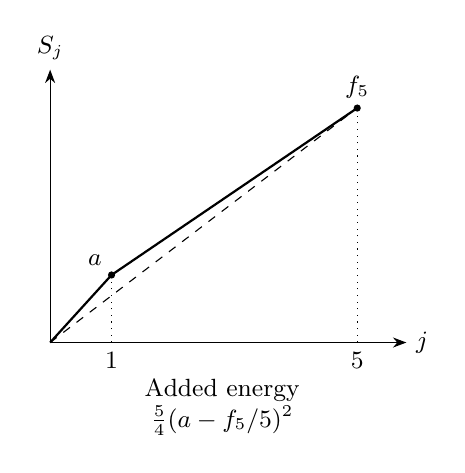
\begin{tikzpicture}[x=.78cm,y=1.65cm,>={Stealth[length=1.7mm]},
                    font=\small]
\draw[->] (0,0)--(5.8,0) node[right]{\(j\)};
\draw[->] (0,0)--(0,2.1) node[above]{\(S_j\)};
\draw[dashed] (0,0)--(5,{sqrt(5)-.61/sqrt(2)});
\draw[thick] (0,0)--(1,.52)--(5,{sqrt(5)-.61/sqrt(2)});
\draw[dotted] (1,0)--(1,.52);
\draw[dotted] (5,0)--(5,{sqrt(5)-.61/sqrt(2)});
\fill (1,.52) circle (1.3pt) node[above left]{\(a\)};
\fill (5,{sqrt(5)-.61/sqrt(2)}) circle (1.3pt)
      node[above]{\(f_5\)};
\node[below] at (1,0){\(1\)};
\node[below] at (5,0){\(5\)};
\node[align=center] at (2.8,-.5)
 {Added energy\\\(\frac54(a-f_5/5)^2\)};
\end{tikzpicture}
\end{minipage}\hfill
\begin{minipage}{.50\linewidth}
\centering
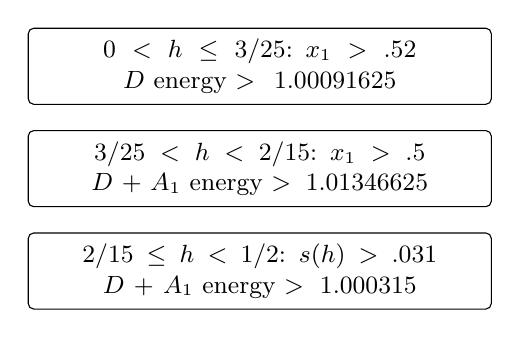
\begin{tikzpicture}[font=\small,
 box/.style={draw,rounded corners=2pt,align=center,
             text width=56mm,inner sep=4pt}]
\node[box] at (0,2.4)
 {\(0<h\le3/25\): \(x_1>.52\)\\
  \(D\) energy \(>1.00091625\)};
\node[box] at (0,1.1)
 {\(3/25<h<2/15\): \(x_1>.5\)\\
  \(D+A_1\) energy \(>1.01346625\)};
\node[box] at (0,-.2)
 {\(2/15\le h<1/2\): \(s(h)>.031\)\\
  \(D+A_1\) energy \(>1.000315\)};
\end{tikzpicture}
\end{minipage}
\caption{The isolated short wall forces an extra first-coordinate
constraint in the same \(D\) projection. The left diagram shows
the reference adjustment; the right lists the exact height cases.
The height boxes are not drawn to scale.}
\label{fig:D23gain}
\end{figure}

\section{The finite forest gives the global bound}\label{sec:global}

We now prove Theorem~\ref{thm:main} from the component estimates above,
without importing a predecessor numerical dimension conclusion.
Suppose \(25\le n\le29\). Call an \(A\)
component of rank at least \(7\), or \(B,D\) of rank at least \(9\),
\emph{dominant}.

If there is none, every rank pays its strict ordinary rank$/14$
cost, except for the alternatives in \eqref{eq:debits}.
Discarding a possible short \(A_1\) gives total energy
\(>(n-1)/14>1\). A rank-two defect gives
\(>9/100+(n-2)/14>1\). Thus a dominant block exists.
Every dominant block pays more than \(1/2\), so there is exactly
one. Only now are all its spectators ordinary apart from the
single permitted debit. Write its rank as \(r\), their total rank
as \(S=n-r\). The three spectator lower bounds are
\begin{equation}\label{eq:spectators}
 \frac S{14},\qquad \frac{S-1}{14},\qquad
 \frac9{100}+\frac{S-2}{14}.
\end{equation}
Empty ordinary sums mean zero. In particular, for a sole rank-two
defect strictness comes from that block's own \(>9/100\).

For a dominant \(A\), the half bound first gives \(S\le7\).
Indeed \(S\ge7\) contradicts the norm without a debit, and
\(S\ge8\) does so with either debit. Hence \(r\ge18\), so the
stronger \(5/7\) estimate applies. A second use of
\eqref{eq:spectators} gives \(S\le4\): the ordinary threshold
is \(S=4\), the short-\(A_1\) threshold is \(S=5\), and the
rank-two threshold at \(S=5\) pays
\[
 5/7+9/100+3/14=713/700>1.
\]
Thus \(r=n-S\ge21\), contrary to the \(A\) cap20.

For dominant \(B,D\), the \(9/14\) floor gives \(S\le5\) and
therefore \(r\ge20\). The caps leave \(r\le22\) for \(B\) and
\(r\le23\) for \(D\). If \(r=20,21\), \eqref{eq:prefixrows}
gives energy \(>.90\) and \(S\ge4\). Even after discarding a short
\(A_1\), three ordinary ranks pay \(>3/14>.10\); a rank-two
defect is stronger. If \(r=22,23\), the energy is \(>.94\) and
\(S\ge2\). One retained ordinary rank pays \(>1/14>.06\);
if instead the spectators are solely a defect, that block pays
\(>.09>.06\). The fully ordinary cases are stronger.
All possibilities contradict \eqref{eq:energy}.

Dimensions \(25\) through \(29\) are therefore impossible.
Vinberg's published ceiling29 excludes all higher dimensions
\cite{Vin84}. It remains to exclude dimension24.

\begin{lemma}[The dimension-twenty-four frontier]\label{lem:frontier24}
At a farthest vertex in dimension24, the preceding bookkeeping
leaves only \(A_{20}\) with four spectator ranks and a permitted
debit, or \(D_{23}\) with one isolated short \(A_1\) of type I.
\end{lemma}
\begin{proof}
Existence and uniqueness of a dominant component follow by the
same norm calculation, which already holds in dimension24.
For a dominant \(A\), the half bound gives \(S\le7\) and hence
\(r\ge17\). The \(5/7\) bound then gives \(S\le4\), so the
cap20 forces \(r=20,S=4\). Fully ordinary spectators would already
give energy \(>5/7+4/14=1\), leaving a permitted debit.
For dominant \(B,D\), \(S\le5\) gives \(r\ge19\).
For \(B,D\) ranks \(19,20,21,22\), the generic theorem's respective
prefix bounds are \(>.88864,.90715,.9240775,.9401975\);
these and the remaining ordinary ranks exclude all their debit
cases. The B cap22 and D cap23 leave only \(D_{23},S=1\).
An ordinary \(A_1\) costs more than the remaining \(.06\).
A rank-two defect and type J both require two ranks, so the
sole spectator is isolated type I.
\end{proof}

The first frontier is excluded by Proposition~\ref{prop:A20}.
After discarding one short \(A_1\), its other three spectator ranks
still pay \(>3/14\), so total energy is \(>11/14+3/14=1\).
For a rank-two defect, the cost is
\[
 11/14+9/100+2/14=713/700>1.
\]
The other frontier is exactly Proposition~\ref{prop:D23I}.
Thus dimension24 is impossible too. This completes
Theorem~\ref{thm:main}. It makes no claim of sharpness, an improved
arithmetic bound, or a new compact example.

\appendix
\section{Supporting derivations and verification scope}\label{app:map}

The proof above integrates the supporting written arguments into one
exposition. The following correspondence is a guide to those derivation
families, not a list of additional mathematical assumptions.
\begin{center}\small
\begin{tabular}{p{.26\linewidth}p{.64\linewidth}}
\toprule
Part of this paper & Supporting derivation family\\ \midrule
Sections~\ref{sec:geometry}--\ref{sec:ordinary}&
Actual mixed replacements and reciprocal shadows; universal small-component
costs; the short-$A_1$ and isolated rank-two debit arguments.\\
Proposition~\ref{prop:BDnine}&
Complete low-index common-pair lists, the native-seven actual dual foot,
and the fixed positive three-pair inequality.\\
Proposition~\ref{prop:caps}&
Foreign-pressure clearing, bulk and short-tail continuation,
actual two-cap replacements, and the $A_{21}$ plateau certificate.\\
Section~\ref{sec:largeA}&
Rank-seven base, uniform half and five-sevenths pressures,
and the stronger $A_{20}$ four-foot argument.\\
Sections~\ref{sec:prefix}--\ref{sec:D23}&
Generic classical prefix interpolation and the coupled isolated-$A_1$
obstruction.\\
Section~\ref{sec:global}&
The dimension-$24$ frontier and its two final exclusions.\\ \bottomrule
\end{tabular}\end{center}

Exact source versions, individual contribution statements, mathematical
review records and source-integrity records are preserved in the project
proof map, \path{docs/compact_farthest_vertex_bounds_proof_map_20261020.md},
and its immutable source packet,
\path{results/compact_farthest_vertex_dimension23_packet_20261020.json}.
No earlier packet or review is changed by the present integration.
Several feet and interpolation estimates were derived jointly before
outside-author reading; repeated derivations are not counted as
independent discoveries.

The accompanying proof-assistant modules verify selected accounting
implications with the component estimates as explicit premises.
They do not formalize the Lorentz geometry, the finite continuation
classifications, or the component energy proofs. The proof of the
theorem is the written argument above, from the geometric and
classification inputs stated in Section~\ref{sec:scope}; source
integrity checks and typesetting serve different purposes.

\begin{thebibliography}{9}
\bibitem{Vin84}
E.~B. Vinberg,
\emph{The absence of crystallographic groups of reflections in
Lobachevsky spaces of large dimension},
Trudy Moskov. Mat. Obshch. \textbf{47} (1984), 68--102;
English translation, Trans. Moscow Math. Soc. (1985), 75--112.
\href{https://www.mathnet.ru/eng/mmo444}{Primary bibliographic record}.

\bibitem{Vin85}
E.~B. Vinberg,
\emph{Hyperbolic reflection groups},
Russian Math. Surveys \textbf{40}:1 (1985), 31--75,
\href{https://doi.org/10.1070/RM1985v040n01ABEH003527}
{doi:10.1070/RM1985v040n01ABEH003527}.
\end{thebibliography}
\end{document}
